%%%%%%%%%%%%%%%%%%%%%%%%%%%%%%%%%%%%%%%%
% Masters/Doctoral Thesis 
% LaTeX Template
% Version 1.43 (17/5/14)
%
% This template has been downloaded from:
% http://www.LaTeXTemplates.com
%
% Original authors:
% Steven Gunn 
% http://users.ecs.soton.ac.uk/srg/softwaretools/document/templates/
% and
% Sunil Patel
% http://www.sunilpatel.co.uk/thesis-template/
%
% License:
% CC BY-NC-SA 3.0 (http://creativecommons.org/licenses/by-nc-sa/3.0/)
%
% Note:
% Make sure to edit document variables in the Thesis.cls file
%
%%%%%%%%%%%%%%%%%%%%%%%%%%%%%%%%%%%%%%%%%

%----------------------------------------------------------------------------------------
%	PACKAGES AND OTHER DOCUMENT CONFIGURATIONS
%----------------------------------------------------------------------------------------

\documentclass[11pt, oneside]{Thesis} % The default font size and one-sided printing (no margin offsets)

\graphicspath{{Pictures/}} % Specifies the directory where pictures are stored
\usepackage{hyperref}
\usepackage{enumerate}
\usepackage{float}
\usepackage{natbib} % Use the natbib reference package - read up on this to edit the reference style; if you want text (e.g. Smith et al., 2012) for the in-text references (instead of numbers), remove 'numbers' 
\hypersetup{urlcolor=blue, colorlinks=true} % Colors hyperlinks in blue - change to black if annoying
\title{\ttitle} % Defines the thesis title - don't touch this

\begin{document}

\frontmatter % Use roman page numbering style (i, ii, iii, iv...) for the pre-content pages

\setstretch{1.3} % Line spacing of 1.3

% Define the page headers using the FancyHdr package and set up for one-sided printing
\fancyhead{} % Clears all page headers and footers
\rhead{\thepage} % Sets the right side header to show the page number
\lhead{} % Clears the left side page header

\pagestyle{fancy} % Finally, use the "fancy" page style to implement the FancyHdr headers

\newcommand{\HRule}{\rule{\linewidth}{0.5mm}} % New command to make the lines in the title page
\newcommand{\avg}[1]{\langle{#1}\rangle}
\newcommand{\nscatt}{\langle N_{\rm scatt}\rangle}
\newcommand{\ly}{{\ifmmode{{\rm Ly}\alpha~}\else{Ly$\alpha$~}\fi}}
\newcommand{\hMpc}{{\ifmmode{h^{-1}{\rm Mpc}}\else{$h^{-1}$Mpc }\fi}}
\newcommand{\hGpc}{{\ifmmode{h^{-1}{\rm Gpc}}\else{$h^{-1}$Gpc }\fi}}
\newcommand{\hmpc}{{\ifmmode{h^{-1}{\rm Mpc}}\else{$h^{-1}$Mpc }\fi}}
\newcommand{\hkpc}{{\ifmmode{h^{-1}{\rm kpc}}\else{$h^{-1}$kpc }\fi}}
\newcommand{\hMsun}{{\ifmmode{h^{-1}{\rm{M_{\odot}}}}\else{$h^{-1}{\rm{M_{\odot}}}$}\fi}}
\newcommand{\hmsun}{{\ifmmode{h^{-1}{\rm{M_{\odot}}}}\else{$h^{-1}{\rm{M_{\odot}}}$}\fi}}
\newcommand{\Msun}{{\ifmmode{{\rm {M_{\odot}}}}\else{${\rm{M_{\odot}}}$}\fi}}
\newcommand{\msun}{{\ifmmode{{\rm {M_{\odot}}}}\else{${\rm{M_{\odot}}}$}\fi}}
\newcommand{\lya}{{Lyman $\alpha$~}}
\newcommand{\clara}{{\texttt{CLARA}}~}
\newcommand{\rand}{{\ifmmode{{\mathcal{R}}}\else{${\mathcal{R}}$ }\fi}}
\newcommand{\hs}{{\hspace{1mm}}}
\newcommand{\kms}{{\ifmmode{{\mathrm{\,km\ s}^{-1}}}\else{\,km~s$^{-1}$}\fi}}

% PDF meta-data
\hypersetup{pdftitle={\ttitle}}
\hypersetup{pdfsubject=\subjectname}
\hypersetup{pdfauthor=\authornames}
\hypersetup{pdfkeywords=\keywordnames}

%----------------------------------------------------------------------------------------
%	TITLE PAGE
%----------------------------------------------------------------------------------------

\begin{titlepage}
\begin{center}

\textsc{\LARGE Universidad de los Andes}\\[1.5cm] % University name


\includegraphics[scale=0.5]{logoUniandes.png}\\[1.5cm]
\textsc{\Large Master Thesis}\\[0.5cm] % Thesis type

\HRule \\[0.4cm] % Horizontal line
{\huge \bfseries The effect of gas bulk rotation on the morphology of the Lyman $\alpha$ line}\\[0.4cm] % Thesis title
\HRule \\[1.5cm] % Horizontal line
 
\begin{minipage}{0.4\textwidth}
\begin{flushleft} \large
\emph{Author:}\\
{Juan Nicolas Garavito Camargo} % Author name - remove the \href bracket to remove the link
\end{flushleft}
\end{minipage}
\begin{minipage}{0.4\textwidth}
\begin{flushright} \large
\emph{Supervisor:} \\
{Dr. Jaime E. Forero Romero} % Supervisor name - remove the \href bracket to remove the link  
\end{flushright}
\end{minipage}\\[3cm]


 
\large \textit{A thesis submitted in fulfilment of the requirements\\ for the degree of \degreename}\\[0.3cm] % University requirement text
\textit{in the}\\[0.4cm]
Astronomy group\\Physics Department\\[2cm] % Research group name and department name
 
{\large \today}\\[4cm] % Date
%includegraphics[scale=0.5]{logoUniandes.png} % University/department logo - uncomment to place it
 
\vfill
\end{center}

\end{titlepage}

%----------------------------------------------------------------------------------------
%	DECLARATION PAGE
%	Your institution may give you a different text to place here
%----------------------------------------------------------------------------------------

%\Declaration{

%\addtocontents{toc}{\vspace{1em}} % Add a gap in the Contents, for aesthetics

%I, \authornames, declare that this thesis titled, '\ttitle' and the work presented in it are my own. I confirm that:

%\begin{itemize} 
%\item[\tiny{$\blacksquare$}] This work was done wholly or mainly while in candidature for a research degree at this University.
%\item[\tiny{$\blacksquare$}] Where any part of this thesis has previously been submitted for a degree or any other qualification at this University or any other institution, this has been clearly stated.
%\item[\tiny{$\blacksquare$}] Where I have consulted the published work of others, this is always clearly attributed.
%\item[\tiny{$\blacksquare$}] Where I have quoted from the work of others, the source is always given. With the exception of such quotations, this thesis is entirely my own work.
%\item[\tiny{$\blacksquare$}] I have acknowledged all main sources of help.
%\item[\tiny{$\blacksquare$}] Where the thesis is based on work done by myself jointly with others, I have made clear exactly what was done by others and what I have contributed myself.\\
%\end{itemize}
 
%Signed:\\
%\rule[1em]{25em}{0.5pt} % This prints a line for the signature
 
%Date:\\
%\rule[1em]{25em}{0.5pt} % This prints a line to write the date
%}

%\clearpage % Start a new page

%----------------------------------------------------------------------------------------
%	QUOTATION PAGE
%----------------------------------------------------------------------------------------

\pagestyle{empty} % No headers or footers for the following pages

\null\vfill % Add some space to move the quote down the page a bit

\textit{``It would obviously be rewarding if our current theoretical
ideas are confirmed by future observations, but it might be even more
exciting if these ideas are modified."}

\begin{flushright}
Abraham Loeb
\end{flushright}

\vfill\vfill\vfill\vfill\vfill\vfill\null % Add some space at the bottom to position the quote just right

\clearpage % Start a new page

%----------------------------------------------------------------------------------------
%	ABSTRACT PAGE
%----------------------------------------------------------------------------------------

\addtotoc{Abstract} % Add the "Abstract" page entry to the Contents

\abstract{\addtocontents{toc}{\vspace{1em}} % Add a gap in the Contents, for aesthetics

In this thesis the effect of gas bulk solid body rotation on 
the morphology of the Lyman $\alpha$ emission line of galaxies
is studied. To this aim radiative transfer simulations 
were implemented for spherical galaxies rotating
in the range $0-300$ \kms and neutral Hydrogen optical depths in the
range $\tau_{\rm H}=10^{5}-10^{7}$. This is studied for the cases of central 
Lyman $\alpha$ photons emission and an homogeneous emission inside
the homogeneous mixture of dust and hydrogen. 
The main result is that rotation increases the width of the line and the flux at the 
center of the line. Rotation also introduces a dependence of the
line morphology with viewing angle.
Due to the fact that rotation does not induce any spatial 
anisotropy in the integrated line flux, the escape fraction 
or the average number of scatterings an analytic approximation for 
the viewing-angle dependence of the emerging spectrum, 
as a function of rotational velocity is derived.
}

%\clearpage % Start a new page

%----------------------------------------------------------------------------------------
%	ACKNOWLEDGEMENTS
%----------------------------------------------------------------------------------------

%\setstretch{1.3} % Reset the line-spacing to 1.3 for body text (if it has changed)

%\acknowledgements{\addtocontents{toc}{\vspace{1em}} % Add a gap in the Contents, for aesthetics

%I feel very gratefull with the departament of physics of the Andes Univserity
%for providing a confortable and motivating atmosphere. In which learning 
%and devloping new skills is very .. I also want to thank the astronomy 
%group leading by Dr. Jaime Forero in which\ldots

%\clearpage % Start a new page

%----------------------------------------------------------------------------------------
%	LIST OF CONTENTS/FIGURES/TABLES PAGES
%----------------------------------------------------------------------------------------

\pagestyle{fancy} % The page style headers have been "empty" all this time, now use the "fancy" headers as defined before to bring them back

\lhead{\emph{Contents}} % Set the left side page header to "Contents"
\tableofcontents % Write out the Table of Contents

\lhead{\emph{List of Figures}} % Set the left side page header to "List of Figures"
\listoffigures % Write out the List of Figures

\lhead{\emph{List of Tables}} % Set the left side page header to "List of Tables"
\listoftables % Write out the List of Tables

%----------------------------------------------------------------------------------------
%	ABBREVIATIONS
%----------------------------------------------------------------------------------------

%\clearpage % Start a new page

%\setstretch{1.5} % Set the line spacing to 1.5, this makes the following tables easier to read

%\lhead{\emph{Abbreviations}} % Set the left side page header to "Abbreviations"
%\listofsymbols{ll} % Include a list of Abbreviations (a table of two columns)
%{
%\textbf{LAH} & \textbf{L}ist \textbf{A}bbreviations \textbf{H}ere \\
%\textbf{Acronym} & \textbf{W}hat (it) \textbf{S}tands \textbf{F}or \\
%}

%----------------------------------------------------------------------------------------
%	PHYSICAL CONSTANTS/OTHER DEFINITIONS
%----------------------------------------------------------------------------------------

%\clearpage % Start a new page

%\lhead{\emph{Physical Constants}} % Set the left side page header to "Physical Constants"

%\listofconstants{lrcl} % Include a list of Physical Constants (a four column table)
%{
%Speed of Light & $c$ & $=$ & $2.997\ 924\ 58\times10^{8}\ \mbox{ms}^{-\mbox{s}}$ (exact)\\
% Constant Name & Symbol & = & Constant Value (with units) \\
%}

%----------------------------------------------------------------------------------------
%	SYMBOLS
%----------------------------------------------------------------------------------------

%\clearpage % Start a new page

%\lhead{\emph{Symbols}} % Set the left side page header to "Symbols"

%\listofnomenclature{lll} % Include a list of Symbols (a three column table)
%{
%$a$ & distance & m \\
%$P$ & power & W (Js$^{-1}$) \\
% Symbol & Name & Unit \\

%& & \\ % Gap to separate the Roman symbols from the Greek

%$\omega$ & angular frequency & rads$^{-1}$ \\
%% Symbol & Name & Unit \\
%}

%----------------------------------------------------------------------------------------
%	DEDICATION
%----------------------------------------------------------------------------------------

\setstretch{1.3} % Return the line spacing back to 1.3

\pagestyle{empty} % Page style needs to be empty for this page

\dedicatory{To my parents: Vilma \& Edgar} % Dedication text

\addtocontents{toc}{\vspace{2em}} % Add a gap in the Contents, for aesthetics

%----------------------------------------------------------------------------------------
%	THESIS CONTENT - CHAPTERS
%----------------------------------------------------------------------------------------

\mainmatter % Begin numeric (1,2,3...) page numbering

\pagestyle{fancy} % Return the page headers back to the "fancy" style

% Include the chapters of the thesis as separate files from the Chapters folder
% Uncomment the lines as you write the chapters

% Introduction

\chapter{Introduction} % Main chapter title

\label{sec:intro} % For referencing the chapter elsewhere, use \ref{Chapter1} 

\lhead{\emph{Introduction}} % This is for the header on each page - perhaps a shortened title

\section{\emph{Motivation}}

It is astonishing how much we can learn from observing and 
contemplating the Universe. All this knowledge of the Universe
led to a better comprehension of the dynamics of the Universe itself 
and how these components such as galaxies, interstellar/intergalactic
medium and stars have been evolved in time. These theories don't have
just an academic impact society has faced different changes of 
paradigm due to these scientific achievements. And hopefully this
knowledge of nature can help us in the path to a modern 
sustainable society with consciousness of our place and role 
in the Universe.  

Astronomy is unique in the sense that there is only one Universe 
to observe. Due to the expanding nature of the Universe and 
that the speed of light is finite, observations of the farther 
regions of the Universe are also from the youngest stages of the Universe.
This allows to observe the evolution of the Universe during redshift.

There are two techniques to measure the radiation coming from the 
Univserse; photometry, spectroscopy and polarimetry. Photometric observations measure 
the flux of astronomical objects in different filters. This allows to derive quantities 
such as the luminosity and the temperature. On the other hand spectroscopic observations 
allow to study in deep detail
the spectra of astronomical objects, in particular the spectra of 
galaxies reveal properties such as the population of stars in the galaxy, the
redshift, the elements that constitute these objects, the characteristics 
of the insterstellar medium and many more.

In particular the Lyman$\alpha$ emission line is a useful 
tool to detect star forming galaxies at high redshift, specially 
at $z>2$ which is when the line is shifted to the optical frame. But 
as discussed in \S\ref{sec:resonant} the morphology of the line 
is substantially affected
by the gas kinematics and distribution, the interstellar gas (IGM)
 and by the dust. 

Understanding the morphology of the \ly line is a crucial endeavour 
to understand deeply the properties of galaxies at high redshift. To this aim 
computer simulations are extremely useful, models of these properties 
can be simulated to create synthetic profiles that can be compared
with the observations. 

This is an important era to study these high redshift galaxies. Computer 
simulations techniques have been improved and more powerful facilites are
now available. Also a new generation of telescopes are being constructed,
these telescopes will have the power to observe more deeply into the sky, 
and new high redshift galaxies are going to be discovered. All these  
improve our understanding of the highredshift Universe. 



\section{\emph{Historical Remarks}}

The emission of the \ly line in galaxies was first predicted by 
\citep{PartridgePeebles} in their work they suggest that the \ly luminosity
could increase the luminosity of the galaxies at high redshift, and that 
it could be detected by the telescopes. 

By the same epoch the radiative transfer theory in \ly systems started to be
 studied \citep{Osterbrock62, Adams72, Harrington73, Neufeld90}
 it can be seen as a diffusion process if it is carried out in 
 an optically thick medium. It means that \ly photons propagating 
in a medium are diffusing in space and in wavelenght from the line center.   
Because of the complexity of these systems an analytical solution 
can only be carried out in simplified systems. 


Almost tree decades later \citep{DjorgovskiThomson92} detected the first \ly 
emitter galaxy (LAE) since then hundreds of galaxies has been  
observed at redshifts $z>2$. There is a confirmed LAE at $z=8.6$ 
by \citep{Lenhert2010} and candidates up to $z\sim12$ by \citep{Brammer13}. 
The \ly line has the potential to be a tool to confirm galaxies at the highest 
redshifts. 

Despite all these observational efforts to fully understand the radiative
transfer (RT) of the \ly line numerical simulations started to be performed.
\citep{DijkstraKramer, Laursen09, Verhamme06, CLARA}
in order to understand more realistic situations.

More recently various teams \citep{Mas-Hesse09,LARS} have
observed nearby galaxies with the Hubble Space Telescope with the
aim to have better spectra and images of the HI distribution 
and kinematics. These new data now can be compared with the numerical 
models developed.

 

\section{\emph{The Lyman $\alpha$ line in astronomy}}\label{sec:lyuses}

The Lyman $\alpha$ (hereafter Ly$\alpha$) emission line is a consequence of the 
transition 
from the first excited level to the ground level of the electron
in the Hydrogen atom. When the electron undergoes such transition 
a photon is emitted with an energy of $13.6eV$ which corresponds to 
a rest wavelenght of $1215.67 \AA$. 

This transition is very common in the Universe due to the high abundance
of hydrogen. Two main mechanisms end up in \ly radiations: Recombination 
processes and collisional events of Hydrogen atoms, UV stellar radiation
from star regions (Recombination), Gravitational 
cooling (Collisional) and UV background radiation (Recombination). The interested
reader could read \citep{LaursenPhD} and references within for
more details. 

The detection of the \ly line has been broadly studied and has multiple 
applications in extragalactic astronomy:

\begin{itemize}
\item {\bf{Detection of high $z$ galaxies:}} One of the most used 
methods to detect high redshift galaxies is finding the \ly emission 
line using narrow band imaging or spectroscopy. With these methods 
hundreds of galaxies has been detected. This 
allow to study the properties of the high redshift Universe such as
the large scale structure. 
 
\item {\bf{Galaxy formation and evolution:}} Observed LAEs at different
reshifts has allowed to derive the Lumimosity Functions (LFs) of LAEs, 
for this aim a good knowledge of the escape fracition of 
photons is requiered $f_{esc}$ see \S \ref{sec:ef} for details on the escape 
fraction of \ly photons. As consequence the observed LAEs LFs enhance a
better understanding of the galaxy formation processes. 

\item {\bf{Reionization:}} The Epoch of Reionization (EoR) is an important
period of the Universe, in which the neutral cold HI gas reionize to 
become a hot gas. There is evidence from CMB measurements that 
the EoR must start at $z >> 11$ and should end up at $z\sim5$. During this 
epoch the intergalactic medium (IGM) became opaque to the \ly radiation 
outcoming from the galaxies. LAEs has also shown to be 
very useful in constraining the time at which the EoR ends. 
For a complete recent review please see \citep{review} and references
within.
 
\end{itemize}


\section{Units, Quantities \& Definitions}

Through this work we will use some units and quantities very popular in 
this area. For clarity here we briefly define and review this 
quantities and units.

\subsection{Optical depth and Column Density}

The optical depth $\tau$ is a measure of the "transparency" of the medium
in which the photons are propagating, $\tau$ is defined as:

\begin{equation}
d\tau = \alpha dr
\end{equation}

Where $\alpha$ is the absorption coefficient defined as:

\begin{equation}
\dfrac{dI}{dr} = -\alpha I
\end{equation}

From these definitions we can now define the "thickness" of the medium.
If $\tau > 1$ we said that the medium is optically thick and this means
that a photon with frequency $\nu$ cannot go through the medium without been
absorbed. If $\tau < 1$ the medium is optically thin and the photon
could be pass through the medium without been absorbed.

The optical depth measure the distance from the source
of photons to the surface of the medium. It is also very common 
to express the amount of gas between the \ly source and the surface
in terms of the Hydrogen column density 
$N_{HI}$ which is related to the optical depth by $N_{HI} = \tau/\sigma$
where $\sigma$ is the Hydrogen atom cross section. 

\subsection{\ly line profile units}

The frequency $\nu_{\alpha}$ of a \ly photon in rest frame is
$2.46\times 10^{15}Hz$,
there are two new variables $x, V$ in which the frequency of 
the \ly alpha photons may be presented in the literature.

The first is a dimensionless variable $x$ defined as:

\begin{equation}\label{eq:x}
x   \equiv \dfrac{(\nu -\nu_{\alpha})}{\Delta \nu_D}
\end{equation}

Where $\nu$ is the frequency in the observer frame,
$\nu_D$ is the broadening of the line due to the thermal
velocity of the Hydrogen atoms $v_{th}$. This velocity can be derived
assuming that the Hydrogen gas is in thermal equilibrium
and follows a Maxwellian distribution. In thermal equilibrium
we get:

\begin{equation}
\dfrac{m_H v_{th}}{2} = K_B T 
\end{equation}

Where $m_H$ is the Hydrogen atom mass, $K_B$ the Boltzmann constant and $T$
the temparature in Kelvins, the expression for $v_{th}$ is then:

\begin{equation}
v_{th} = \sqrt{\dfrac{2 K_B T}{m_H}} = 128.5 T^{1/2}\dfrac{m}{s}
\end{equation}

The Doppler shift due to $v_{th}$ would be:

\begin{equation}
\nu'= (1 - \dfrac{\vec{v_{th}}\cdot\vec{n}}{c})\nu_{\alpha}
\end{equation}

Which can be expressed in terms of $\Delta \nu_D$ as:

\begin{equation}
\nu_{\alpha} - \nu' = \Delta\nu_D =  \dfrac{\vec{v_{th}}\cdot\vec{n}}{c} \nu_{\alpha}
\end{equation}

It is also common to express the line profile in terms of the velocity $V$
making use of Eq.\ref{eq:x}:

\begin{equation}
V = xv_{th} = \dfrac{\nu - \nu_{\alpha}}{\nu_{\alpha}}c
\end{equation}

\subsection{Average number of scatterings $N_{scatt}$}

The path of a \ly photon inside an {\bf{optically thick}}
HI medium is resonant this is explained in more detail 
in \S \ref{sec:resonant}. It basically means that the \ly photon
after been emitted by the source is absorbed by an H atom
and re-emitted in a time scale of $\sim 10^{-9}$ s.
For this reason, this process is commonly referred as
a scattering process. The total number of scatterings
is denoted as $N_{scatt}$ and it is proportional to
$\tau^2$.



\subsection{Resonant scattering}\label{sec:resonant}

Hydrogen is the most abundant element in the Universe furthermore
the \ly line is a very common line. However the transmission of these
\ly  photons through the Hydrogen clouds is not trivial. There 
are two main aspects that heavily influence the morphology of the line.

Imagine that there is one Hydrogen atom which emits 
a \ly photon in the middle of a cloud of HI. 
The \ly photon will be absorbed and re-emitted from 
the Hydrogen atom. This process will end up in a random walk in the space,
and the photon can escape the cloud at any point in of the surface, see 
Fig.\ref{fig:rw}.\\

\begin{figure}
\begin{center}
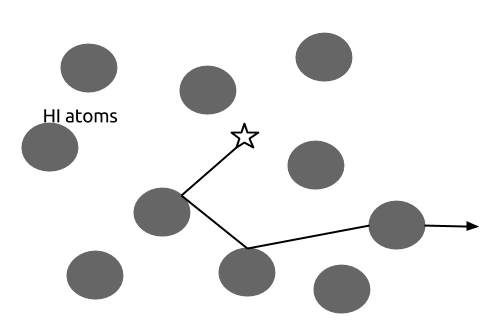
\includegraphics[scale=0.4]{Figures/randomwalk.png}
\end{center}\caption{Scattering scheme of a \ly photon in a HI medium
(The star represent a \ly source and the solid line represents the path that
the \ly photon follow before scaping the cloud).\label{fig:rw}}
\end{figure}


In the previous situation all the Hydrogen atoms were in rest, if the atoms
present proper motions there would be a Doppler shift Fig.\ref{fig:xshift}. 
If an atom have a velocity $v$ an emit a \ly photon in the direction 
opposite to the movement the \ly photon 
would be redshifted. But if it is emitted in the same direction of movement the
\ly photon would be blueshifted.    

\begin{figure}[H]
\begin{center}
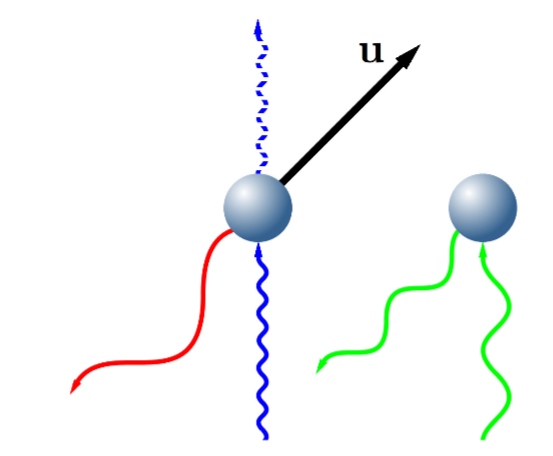
\includegraphics[scale=0.4]{Figures/xshift.png}
\end{center}\caption{Scheme of the frequency shift. Left: Rest frame, Because 
of the velocity $u$ of the atom absorb a blue-shifted \ly photon, and emit 
a red-shifted \ly photon. Right HI atom rest frame when all photons have the \ly frequency. (Image credit: Interpereting Lyman $\alpha$ radiation from young, dusty galaxies. By: Peter Laursen, 2010.).\label{fig:xshift}}
\end{figure}


This two effects made ratiave trasnfer inside optically thick medium as a random 
walk in space and frequency. This is why Monte-Carlo methods can be
applyed to this diffusion process.
 
\subsection{Escape fraction}\label{sec:ef}

Dust grains are mainly considered as metals in the ISM, these
metals are formed in stars. At high redshifts where galaxies and 
stars are young the most probable escenario in that supernovae 
enrich the ISM with dust \citep{Kotak09}, in this way the observed 
dust \citep{Coppin09}  at high redshift is explained. 

The effect of dust in the \ly transfer inside the ISM is that 
dust grains can absorb (destroy) or scatter \ly photons. The 
probability of these events is given by the 'albedo' $A$ defined as:

\begin{equation}
A = \dfrac{\sigma_{scatt}}{\sigma_{dust}}
\end{equation}

Where $\sigma_{scatt}$ is the total cross section for scattering 
and $\sigma_{dust}$ for absorption. $\sigma_{dust}$ can be derived from 
dust properties see \citep{Laursen09}. 

There are two approaches to the modelling of dust in the \ly RT process.
As a first approximation the dust distribution is taken as an homogeneous distribution 
in the HI region and 
the \ly photons can be absorbed by the dust or scattered. A more
sophisticated situation is that the medium follows a clumpy distribution
of dust in which \ly photons are more likely to scatter with the 
clumps rather than absorbed \citep{Laursen13}. To quantify the effect of 
the dust the ratio
of \ly photons observed (\ly alpha photons who manage to scape from the medium) 
over the \ly photons emitted define a quantity call the {\bf{escape fraction}} $f_{esc}$. 

It is worth pointing out that the analytical
description of the \ly RT doesn't take into account the presence of
dust. That is also a motivation to include dust in the numerical simulations.
As is explained in more detail in \S \ref{sec:analytic}.  





\section{\emph{Attenuation of the \ly emission line}}

Despite the fact that the \ly line is the strongest emission line in 
the UV, there were 25 years since the prediction of the \ly line to 
the first observation by \citep{DjorgovskiThomson92}. 
This long absence of the \ly line is what makes this and excited and 
challenging field.

Figure\ref{fig:IGM} shows the outcoming spectra from a galaxy 
at $z \sim 3.5$, the line is double peaked as expected from 
the radiative transfer process in the galaxy. After the encounter
with the inter-galactic medium (IGM) de blue peak is diminished.
Dut to the expansion of the Universe the blue peak 
is shifted to the \ly frequency and the HI in the IGM would absorb
part of this radiation. As a result the observed spectra (right figure)
is asymmetric.   

\begin{figure}[H]
\begin{center}
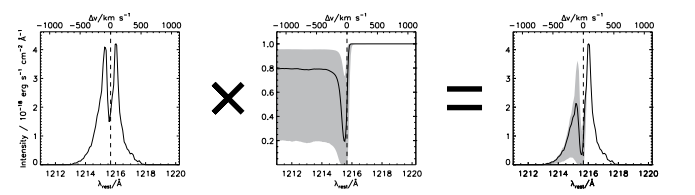
\includegraphics[scale=0.6]{Figures/ISM.png}
\end{center}\caption{The IGM effect on the \ly line. (Image Credit:)\label{fig:IGM}}
\end{figure}


The gas kinematics in the galaxy also plays a mayor role in shaping
the morphology of the line, due to the resonant nature of the line. 
Figure\ref{fig:kulas} show the \ly line
profile for different galaxies at $z \sim 2 - 3$, due to the different
kinematics of those galaxies all the spectra reveals asymmetric profiles 
and some of them are multi-peaked.    


\begin{figure}[H]%\label{fig:kulas}
\begin{center}
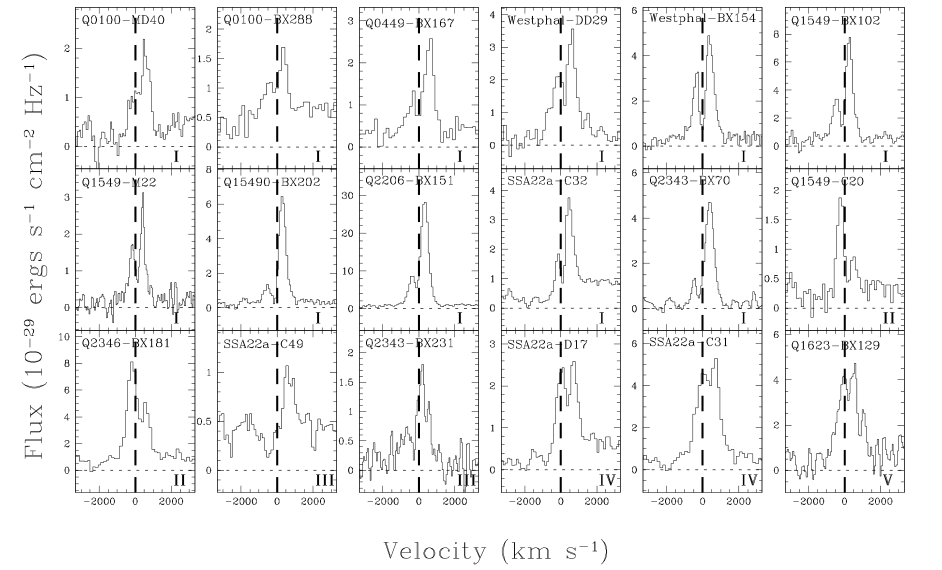
\includegraphics[scale=0.4]{Figures/kulas.png}
\end{center}\caption{Asymmetry and multipeaked \ly line profiles. (Image credit: The kinematics of multiple-peaked \ly emission in star-forming galaxies at $z\sim 2$ - 3. Kulas, K. et al 2011)\label{fig:kulas}
 }
\end{figure}

The presence of dust in galaxies also play an important role, dust as explained
 in \S\ref{sec:ef} could either absorb or scatter \ly photons. As a 
consequence dust mainly diminish the intensity of the \ly line of LAEs. 

Alongside these processes when observing the abundance of LAEs across
the history of the Universe the population of LAEs increases 
with the redshift. But at redshifts $z>6$ the  
abundance of LAEs decrease \citep{Schenker12}. Apparently 
 reionization  is governing at that redshift and the IGM medium 
becomes opaque to \ly radiation.   

All these effects make the \ly line a sensitive line and challenging
to observe at $z>6$ see \citep{Sobral15}, but with valuable information
of the ISM/IGM distribution and kinematics. All these makes de \ly
line a very useful line to explore the extragalactic Universe as
discussed in \S\ref{sec:lyuses}.

  

\section{\emph{Analytical Models}}\label{sec:analytic}

Understanding the \ly line profile requires a theoretical knowledge
about the physics processes involving the radiative transfer. Simplified 
situations have been studied in order to obtain an analytical 
 profile.  In this section, the most relevant 
analytical models are explained in the chronological order in which 
they have been developed. 

The radiative transfer of \ly photons has been studied by several authors
see \citep{RybickiLightman79} for a complete treatment, the Intensity
of \ly photons can be studied via:
 
\begin{equation}\label{eq:RT}
n\cdot\nabla I(\nu, n)= - \alpha_{\nu} I(\nu, n) + j(\nu, n) + \int d\Omega' \int dn' I(\nu', n') R(\nu', \nu, n', n)
\end{equation}

Where $\nu$ is the frequency of the \ly photons. $n$ is the direction 
of the \ly photon. $I(\nu, n)$ is the intensity
of the radiation. $\Omega$ is the solid angle. $R(\nu', \nu, n', n)$ 
is the redistribution function, basically this function which measures 
the probability that a \ly photon with frequency $\nu'$ and direction $n'$
after scatters have a frequency $\nu$ and direction $n$.

The mean density $J_{\nu}$ is defined as:

\begin{equation}\label{eq:J}
J_{\nu} = \dfrac{1}{4\pi}\int I_{\nu}d\Omega
\end{equation}


Using Eq.\ref{eq:J} and following the above steps:

\begin{itemize}
\item In an optically thick medium the dependence on the direction {\bf{$n$}} can 
be neglected.
\item Using a Taylor expansion in ($I(\nu', n')$) in the second term of the right in Eq.\ref{eq:RT} 
\item Replacing the absorption coefficient in terms of the optical depth.
\item $j(\nu, n)=0$ and $\sigma_{dust}=0$
\end{itemize}

Eq.\ref{eq:RT} can be expressed as: 

\begin{equation}\label{eq:RTeq}
\dfrac{dJ(\nu)}{d\tau} = \dfrac{(\Delta \nu_D)^2}{2}\dfrac{\partial}{\partial \nu}\phi(\nu)\dfrac{\partial J(\nu)}{\partial \nu}
\end{equation}

Where $\phi(\nu)$ is a Voigt profile (Combolution of a Gaussian profile  
and Lorentzian profile), this Voigt profile respond to the resonant nature 
of the line. Eq.\ref{eq:RTeq} is a diffusion equation in space and frequency
for the \ly photons in HI clouds. Different authors have solved 
Eq.\ref{eq:RT} in simplified situations that we are going to discuss above. 

\subsection{Infinite Slab with \ly source at the center:}

The first analytical solution to the RT Eq.\ref{eq:RTeq}
was an effort in which different authors made a contribution \citep{Unno55, Osterbrock62, Adams72, Harrington73} and ended with the analytical expression
derived by \citep{Neufeld90} based on the previous works. 

\begin{equation}
J(\tau, x) = \dfrac{\sqrt{6}}{24}\dfrac{x^2}{\sqrt{\pi}a\tau cosh[\sqrt{\pi^3/54}(x^3-x_{in}^3)/a\tau]}
\end{equation}

Where $a$ is the Voigt parameter defined as $a=A/4\pi\Delta \nu_D$. \citep{Harrington73} also show that the maximum intensity of the line is at:

\begin{equation}
x_m = \pm1.066(a\tau)^{1/3}
\end{equation}

And the average number of scatterings is:

\begin{equation}
N_{scatt} = 1.612\tau
\end{equation}

In Fig.\ref{fig:slab} the analytical profile of the slab solution is shown, 
the solid line is the simulated profile reproduced with \citep{CLARA} the code
used in this work.

\begin{figure}[H]
\begin{center}
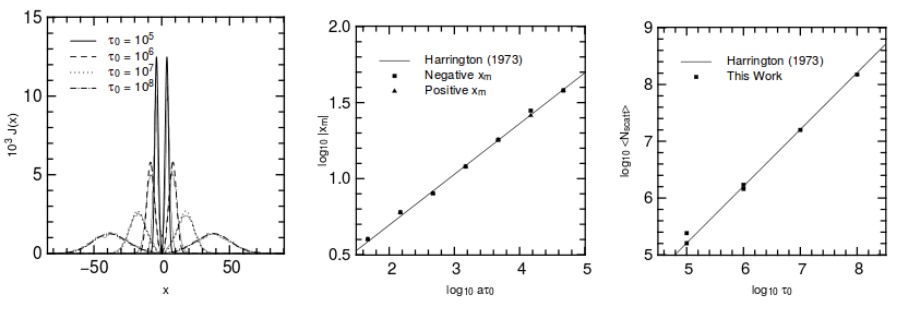
\includegraphics[scale=0.4]{Figures/slab.png}
\end{center}\caption{(left) Analytic profile for a dustless infinite slab with central
\ly sources. (Middle) Maximum peaks position. (Right) Average number of 
scatterings $N_{scatt}$ in function of the optical depth $\tau$.(Image credit:  CLARA's view on the escape fraction of \ly photons in high redshift galaxies. J.E Forero-Romero, et al 2011)\label{fig:slab}}
\end{figure}

\subsection{Spherical solution}

For a spherical gas dustless distribution with central \ly sources \citep{Dijkstra06} has shown that the emergent spectrum is described by the following expression:

\begin{equation}
J(\tau, x) = \dfrac{\sqrt{\pi}}{4\sqrt{6}}\dfrac{x^2}{a\tau (1+cosh[\sqrt{2\pi^3/27}x^3/a\tau])}
\end{equation}

The analytical spectrum of the spherical solution 
is shown in Fig.\ref{fig:sphere} for different optical depths. 

\begin{figure}[H]
\begin{center}
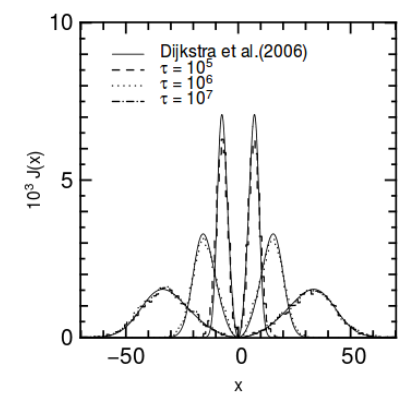
\includegraphics[scale=0.4]{Figures/Sphere.png}
\end{center}\caption{Analytic profile for a dustless sphere with central \ly sources.  (Image credit: CLARA's view on the escape fraction of \ly photons in high redshift galaxies. J.E Forero-Romero, et al 2011)\label{fig:sphere}}
\end{figure}

\subsection{Spherical rotating sphere}

In this work Mark Dijkstra has shown also that an approximate analytical profile
can be derived for a {\bf{rotating spherical distribution}} Eq.\ref{eq:spherero}
with central sources and dustless. This would be the first time that an analytic
al profile is derived for a non-static medium.  

\begin{equation}\label{eq:spherero}
J(x,b,\phi,i)=\frac{\sqrt{\pi}}{\sqrt{24}a\tau_0}\Bigg{(}\frac{(x-x_{\rm
b})^2}{1+{\rm cosh}\Big{[}\sqrt{\frac{2\pi^3}{27}}\frac{|(x
-x_{\rm b})^3|}{a\tau_0}\Big{]}}\Bigg{)}
\end{equation}

\begin{equation}
J(x,i)= \approx 2\pi \int_0^Rdb \hs b
\int_0^{2\pi}d\phi \hs J(x,b,\phi,i)\\ \nonumber
\end{equation}

\section{\emph{Simulated models \& techniques}}

In the Universe most of the galaxies have complicated
geometries (Spirals, irregular) and kinematics that 
can not be resolved analitically. There are two approaches
to understant these complicated properties of galaxies, based
on Monte-Carlo simulations. The first approach is implementing 
the properties of the galaxies, such as: The geometry
of the gas, the kinematics of the gas and the dust. In this 
approach every property is isolated simulated in order
to compute the \ly profiles, escape fractions, average number
of scatterings, position of the maximum peaks among others. 

Realistic galaxy properties in the sense of gas geometry
and kinematics using hydrodynamic simulations. In this 
approach the galaxy can be simulated isolated see \citep{Verhamme12}
or galaxies in the cosmic web can also be studied see\citep{Yajima12}.
The temperature, density and gas velocity fields are obtained from 
the hydrodynamic simulations and then the Monte-Carlo code is 
implemented in order to compute the profile properties.

\subsection{Monte-Carlo approach:}

Monte-Carlo (MC) simulations are broadly used in a variety of 
areas such as science, economy, traffic simulations among 
many more. MC methods are mostly based in the
generation of random numbers that are the core of 
random walks. This is why MC is used to study the
\ly profile. Here we briefly describe how this method 
work. The main thing is that every every \ly photon is simulated
separately in the following scheme, for a detailed description 
please see chapters $6-8$ in \citep{LaursenPhD} .

\begin{itemize}
\item  The temperature (T) is very common to take $T=10^4K$, gas distribution ($\tau$) and kinematics ($V$) is implemented. 

\item Initialize your \ly photon initial position and frequency $x_{in}$

\item Generate a random displacement ($\tau_0$) of the photon in a random 
direction {\bf{$\vec{n}$}}.

\item  Derive the HI atom velocity components from the initial field, 
and generate random components for the thermal movements.

\item  Set the new direction of the \ly photon after scattering.

\item If the \ly photon encounter a dust particle the albedo probability 
would define if the atom is absorbed or scattered. In also common to take $A=1/2$

\item Repeat from step 2 untill the photon reaches the HI surface at $\tau$.  

\end{itemize}

With this method the final frequency $x_{out}$, the average number of scatterings $N_{scatt}$ can be computed for every step in the random walk.


\subsection{Numerical Models of \ly profiles:}

Using the MC method explained above different RT  codes 
\citep{DijkstraKramer, Laursen09, Verhamme06, CLARA}
have been developed in order to understand the effect of the gas kinematics in
the \lya line, expanding/contracting shell/spherical geometries
has been broadly studied \citep{Ahn03,Verhamme06,Dijkstra06}.
Realistic ISM/IGM medium has also been studied, the effect of a clumpy
medium is discussed in \citep{Hansen06}. Anisotropic \ly emission 
has been studied by \citep{Zheng2013}. Realistic expanding mediums 
in cavities has been recently studied by  \citep{Behrens2014} 
Hydrodynamic simulations have studied the outcoming spectra of
LAEs in large scale simulations \cite{Forero12}. 
Recently Monte Carlo codes have been used in hydrodynamic 
simulations to study in detail individual galaxies and galaxies 
in the cosmic web.
\citep{Laursen09,Barnes11,Verhamme12,Yajima12}

Figure \ref{fig:out} shows the effect of outflow/inflow kinematics, 
In the outflow regime photons are blueshifted and the blue part of the line
is stronger than the red part. In the inflow regime the opposite effect
is carried out, the \ly photons are redshifted. 

\begin{figure}[H]%\label{fig:out}
\begin{center}
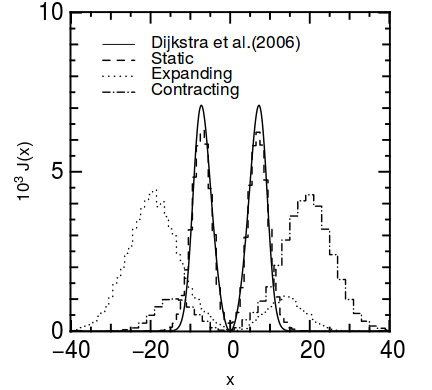
\includegraphics[scale=0.4]{Figures/out.png}
\end{center}\caption{\ly profile of outflows (Expanding medium) dot line, 
and inflows (Contracting) dot-line. (Image credit: CLARA's view on the escape fraction of \ly photons in high redshift galaxies. J.E Forero-Romero, et al 2011)\label{fig:out}
 }
\end{figure}

\section{\emph{This Thesis}}

In this thesis we study the effect of rotation, an intrinsic
 characteristic of galaxies, on the morphology
of the \lya outcoming profile, to this aim we implement a solid body
rotation model in the radiative transfer code \verb+CLARA+ \citep{CLARA}.
All the codes used for the analysis of this work is reproducible
and public available in \href{https://github.com/jngaravitoc/RotationLyAlpha}{github}.

\subsection{The importance of modelling the effect of gas bulk rotation}

Untill now the effect of rotation have never been studied, and this is 
an intrinsic properties of all galaxies. In this work we study for the 
first time the effect of galaxy rotation the morphology of the \ly line.

Modelling the effect of rotation in the morphology of the \ly line, push
further our understanding of the kinematics effects on the \ly line. 
With these models a realistic analysis can be made in observed \ly spectra. 
Now a distinction between the different stages of the gas kinematics
 outflow/inflow, anisotropic \ly emission, shell cavities and now
 rotation is possible.

Deriving and analytic expression for rotation is also important for
the community, computing an analytic solution is more efficient than
making all the radiative transfer simulation. Radiative transfer codes
can be tested against the analytic solution and observed spectra could
be easily fitted  with the model. 

\subsection{Summary of the thesis}

A lot of progress has been done in modelling the \ly line using radiative
transfer codes. Properties of the gas kinematics such as outflows/inflows. 
Geometries such as slabs, spheres, cavities and the propagation of \ly photons
in a clumpy media. In this thesis we study the effect 
of rotation in the morphology of the \ly profile.  

We model a galaxy as a sphere, with an homogeneous mixture of gas and dust. 
We took the rotation velocity, the optical depth, the viewing angle as free
parameters of the model. We also have two different sources of \ly photons:
A central distribution in the galaxy and an homogeneous distribution. 

We quantify the effect of rotation with the following characteristics: 
Escape fraction of \ly photons, the width of the \ly line, the average number
of scatterings of the \ly photons and with the position of the \ly line maximum.

Our main finding is that rotation do have an important effect on the morphology 
of the \ly line. Specially in the width of the line and in the position of the 
maxima. While the average number of scatterings  and the scape
fraction remain constant.

The line broadens proportional to the rotation velocity, and also the flux in 
the middle of the line increases with rotation.

The axis of rotation breaks the symmetry of the system, Althogh 
observers in different viewing angle with respect to the rotation axis
observe the same amount of flux of the \ly profile. But the morphology
of the profile is affected with the observer position, at some angles
the profile is double-peaked and others have single peaked profiles. 
 
 
With these results an approximated analytical solution was derived, 
taking into the account that the radiative transfer inside de gas
cloud is exactly as in the static case. In the sphere surface
a Doppler shift due to the difference velocity of an external 
observer and the surface have to be taken into account.  


\subsection{Future work}


There are two main projects which are based on the results obtained in 
this work. With the aim of testing our model with observations and
improving the kinematic models of the gas by studying two joint effects
such as outflows and rotation.  

\begin{itemize}


\item There are LAEs which are governed by rotation, also 
have approximated spherical geometries and the main \ly sources are in the center. 
With these properties such galaxies have the same properties 
that we studied in this work.  
Fitting \ly line profile in order  to measure the rotational 
velocities of such galaxies would be the direct application 
and test of our model. 

To this aim we are fitting our model using a Marov Chain Monte-Carlo 
method to the observed compact dwarf galaxy \verb+TOL1214-277+\citep{Thuan97, Verhamme15}
. The spectra of this galaxy is shown in Fig.\ref{fig:tol}, 
this galaxy have properties that lead us to derive the rotational 
velocity; it is a compact dwarf galaxy whose geometry can be approximated by a sphere, 
is young and there is no evidence of outflows see \citep{Verhamme15} for a detailed
discussion, in that paper this triple-peaked spectum could not be explained
with the current radiative transfer models. While in our rotation 
model is a common feature to see a triple-peaked spectrum. 

\begin{figure} 
\begin{center}
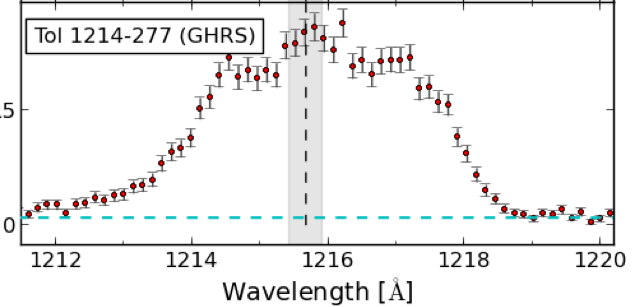
\includegraphics[scale=0.6]{Figures/tol.png}
\end{center}\caption{Tol1214-277 spectra.\label{fig:tol}} 
\end{figure}

\item Despite the fact that outflows have been broadly studied rotation should 
also be present on these galaxies. The joint effect of the two above properties 
should have a direct effect on the morphology of the \lya line. We are 
 combining the effect of rotation followed by an outflow. For the rotation
part we are using our analytic solution and for the outflows
we are using the shell described in \citep{Verhamme12}. 
\end{itemize}

% Chapter Template

\chapter{The effect of gas bulk rotation on the morphology of the \ly line} % Main chapter title

\label{sec:implementation} % Change X to a consecutive number; for referencing this chapter elsewhere, use \ref{ChapterX}

\lhead{\emph{The effect of gas bulk rotation on the morpohlogy of the \ly line}} % Change X to a consecutive number; this is for the header on each page - perhaps a shortened title

%----------------------------------------------------------------------------------------
%	SECTION 1
{\bf{J.N. Garavito-Camargo, J.E Forero-Romero \&  Mark Dijkstra.}}

\section*{abstract}
We present results of radiative transfer calculations to measure the
impact of gas bulk rotation on the morphology of the Lyman $\alpha$
emission line in distant galaxies.
We model a galaxy as a sphere with an homogeneous mixture of dust and
hydrogen at a constant temperature.
These spheres undergo solid-body rotation with maximum velocities in
the range $0-300$ \kms and neutral hydrogen optical depths in the
range $\tau_{\rm H}=10^{5}-10^{7}$.
We consider two types of source distributions in the sphere: central and
homogeneous.
Our main result is that rotation introduces a dependence of the
line morphology with viewing angle and rotational velocity.
Observations with a line of sight parallel to the rotation axis yield
line morphologies similar to the static case.
For lines of sight perpendicular to the rotation axis both the intensity at the line
center and the line width increase with rotational velocity.
Along the same line of sight, the line becomes single peaked at rotational
velocities close to half the line width in the static case.
Notably, we find that rotation does not induce any spatial anisotropy in the integrated line flux, the escape fraction or the average number of scatterings. This is because Lyman $\alpha$ scattering through a rotating solid-body proceeds identical as in the static case. The only difference is the doppler shift from the different
regions in the sphere that move with respect to the observer. This
allows us to derive an analytic approximation for the viewing-angle
dependence of the emerging spectrum, as a function of rotational velocity.

\section{Introduction}
\label{sec:intro}
The detection of strong \ly emission lines has become an essential
method in extra-galactic astronomy to find distant star-forming
galaxies
\citep{PartridgePeebles,Rhoads00,Gawiser2007,Koehler2007,Ouchi08,Yamada2012,Schenker2012,Finkelstein2013}.
The galaxies detected using this method receive the
name of \ly emitters (LAEs).
A detailed examination of this galaxy population has diverse
implications for galaxy formation, reionization and the large scale
structure of the Universe.
Attempts to fully exploit the physical information included in the \ly
line require an understanding of all the physical factors involved in
shaping the line.
Due to the resonant nature of this line, these physical factors
notably include temperature, density and bulk velocity field of the
neutral Hydrogen in the emitting galaxy and its surroundings.
A basic understanding of the quantitative behavior of the \ly line
has been reached through analytic studies in the case of a static
configurations, such as uniform slabs
\citep[][]{Adams72,Harrington73,Neufeld90} and uniform spheres
\citep{Dijkstra06}.
Analytic studies of configurations including some kind of bulk flow
only include the case of a sphere with a Hubble like expansion flow
\citep{LoebRybicki}.
A more detailed quantitative description of the \ly line has been
reached through Monte Carlo (MC) simulations \citep{Auer68,Avery68,Adams72}.
In the last two decades these studies have become popular due to the
availability of computing power.
Early into the 21st century, the first
studies focused on homogeneous and static media
\citep{Ahn00,Ahn01,Zheng02}.
Later on, the effects of clumpy media \citep{Hansen06} and
expanding/contracting shell/spherical geometries started to be studied
\citep{Ahn03,Verhamme06,Dijkstra06}. For a recent review, we refer the interested reader to \citet{review}.
Similar codes have applied these results to semi-analytic models of
galaxy formation \citep{Orsi12, Garel2012} and results of large
hydrodynamic simulations \citep{CLARA,Forero12,Behrens13}.
Recently, Monte Carlo codes have also been applied to the results of
high resolution hydrodynamic simulations of individual galaxies
\citep{Laursen09,Barnes11,Verhamme12,Yajima12}.
Meanwhile, recent developments have been focused on the systematic
study of clumpy outflows \citep{DijkstraKramer} and anisotropic
velocity configurations \citep{Zheng2013}.
The recent studies of galaxies in hydrodynamic simulations
\citep{Laursen09,Barnes11,Verhamme12,Yajima12} have all shown
systematic variations in the \ly line with the viewing angle. These
variations are a complex superposition of anisotropic density
configurations (i.e. edge-on vs. face-on view of a galaxy), the
inflows observed by gas cooling and the outflows included in the
supernova feedback process of the simulation. These bulk flows
physically correspond to the circumgalactic and intergalactic medium
(CGM and IGM). These effects are starting to be studied
in simplified configurations that vary the density and wind
characteristics \citep{Zheng2013,Behrens2014}.
However, in all these efforts the effect of rotation,
which is an ubiquitous feature in galaxies, has not been
systematically studied. The processing of the \ly photons in a
rotating interstellar medium (ISM) must have some kind of impact in
the \ly line morphology.
Performing that study is the main goal of this paper. We investigate for the
first time the impact of rotation on the morphology of the \ly
line. We focus on a simplified system: a spherical gas cloud with
homogeneous density and solid body rotation, to study the line
morphology and the escape fraction in the presence of dust. We base
our work on two independent Monte Carlo based radiative transfer codes
presented in \cite{CLARA} and \cite{DijkstraKramer}.
This paper is structured as follows: In \S \ref{sec:implementation} we
present the implementation of bulk rotation into the Monte Carlo
codes, paying special attention to coordinate definitions. We also
present a short review of how the \ly radiative transfer codes work
and list the different physical parameters in the simulated grid of
models. In \S \ref{sec:results} we present the results of the
simulations, with special detail to quantities that show a
clear evolution as a function of the sphere rotational velocity. In \S
\ref{sec:discussion} we discuss the implications of our results. In
the last section we present our conclusions. The Appendix presents the
derivation of an analytic expression to interpret
the main trends observed in the Monte Carlo simulations.
In this paper we express a photon's frequency in terms of the
dimensionless variable $x\equiv (\nu -\nu_a)/\Delta\nu_{\rm D}$, where
$\nu_{\rm \alpha}=2.46\times 10^{15}$ Hz is the Ly$\alpha$ resonance
frequency, $\Delta\nu_{\rm D} \equiv
\nu_{\alpha}\sqrt{2kT/m_pc^2}\equiv \nu_av_{\rm th}/c $ is the Doppler
broadening of the line which depends on the neutral gas temperature
$T$ or equivalently the thermal velocity
$v_{\rm th}$ of the atoms. We also use the parameter $a$ to define the
relative line width as $a=\Delta\nu_{\alpha}/2\Delta\nu_{\rm D}$,
where $\Delta\nu_{\alpha}$ is the intrinsic linewidth. For the
temperature $T=10^4$K used in our radiative transfer calculations the
thermal velocity is $v_{\rm th}=12.8$\kms.
\section{Models of bulk gas rotation}
\label{sec:implementation}
Describing the kinematics of gas rotation in all generality is a
complex task, specially at high redshift where there is still missing
a thorough observational account of rotation in galaxies beyond
$z>1.0$. Even at low redshifts there is a great
variation in the shape of the rotation curve as observed in HI
emission as a function of the distance to the galaxy center. However
there are two recurrent features. First, in the
central galactic region the velocity increases proportional to the radius,
following a solid rotation behavior. Second, beyond a certain radius
the rotation curve tends to flatten. An ab-initio description of
such realistic rotation curves in simulations depends on having access to
the dynamic evolution of all mass components in the galaxy: stars, gas
and dark matter. Such level of realism is extremely complex to
achieve, specially if one wants to get a systematic description based
on statistics of simulated objects.
Following the tradition of studies of \ly emitting systems,
we implement a model with simplified geometry. We assume that the gas
is homogeneously distributed in a sphere that rotates as a solid body
with constant angular velocity. This simple model will contain only
one free parameter: the linear velocity at the sphere's surface, $V_{\rm
max}$.
\subsection{Detailed Implementation of Rotation}
In the Monte Carlo code we define a Cartesian coordinate system to
describe the position of each photon. The origin of this system
coincides with the center of the sphere and the rotation axis is defined
to be $z$-axis. With this choice, the components of the gas bulk velocity
field, $\vec{v} = v_{x}\hat{i} + v_{y}\hat{j} + v_{z}\hat{k}$, can be
written as
\begin{equation}
v_{x}=-\frac{y}{R}V_{\rm max}, \label{subeq1}
\end{equation}
\begin{equation}
v_{y}=\frac{x}{R}V_{\rm max}, \label{subeq2}
\end{equation}
\begin{equation}
v_{z}=0, \label{subeq3}
\end{equation}
%
where $R$ is the radius of the sphere and $V_{\rm max}$ is the linear
velocity at the sphere's surface. The minus/plus sign in the
$x$/$y$-component of the velocity indicates the direction of
rotation. In this case we take the angular velocity in the same
direction as the $\hat{k}$ unit vector. With these definitions we can
write the norm of the angular velocity as $\omega=V_{\rm max}/R$.
For each photon in the simulation we have its initial position inside
the sphere, direction of propagation $\hat{k}_{\rm in}$ and reduced
frequency $x_{\rm in}$.
The photon's propagation stops once they cross the
surface of the sphere. At this point we store the position, the outgoing direction
of propagation $\hat{k}_{\rm out}$ and the reduced frequency $x_{\rm
out}$. We now define the angle $\theta$ by $\cos\theta = \hat{k}_{\rm out}\cdot
\hat{k}\equiv \mu$, it is the angle of the outgoing photons with
respect to the direction of the angular velocity. We use the variable $\mu$ to
study the anisotropy induced by rotation. Fig. \ref{fig:geometry}
shows the geometry of the problem and the important variables.
\begin{figure}
\begin{center}
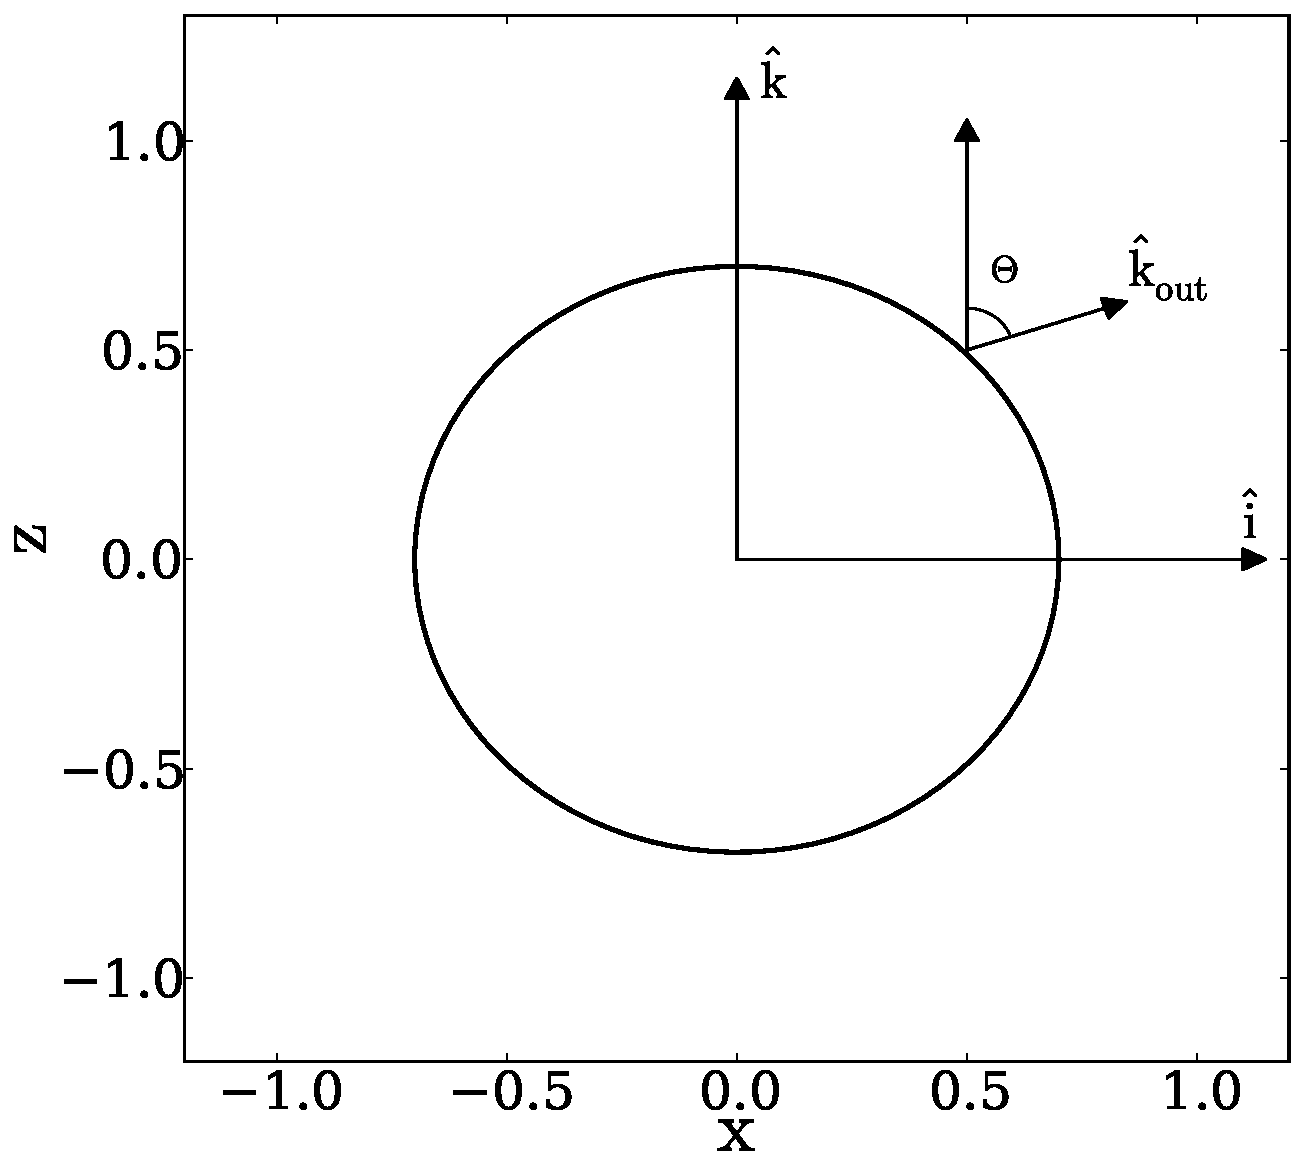
\includegraphics[width=0.4\textwidth]{Figures/f1.pdf}
\end{center}
\caption{Geometry of the gas distribution. The angular velocity vector
is parallel to the unit vector $\hat{k}$. In order to describe the
departures from spherical symmetry we use the polar angle $\theta$
formed by the direction of the outgoing photons with respect to the
$z$-axis. We define define the variable $\mu\equiv\cos\theta$ to
report to present our results. Computing the spectra for photons in
a narrow range of $\mu$ is equivalent to having a line-of-sight
oriented in that direction.
\label{fig:geometry}}
\end{figure}
\begin{figure*}
\begin{center}
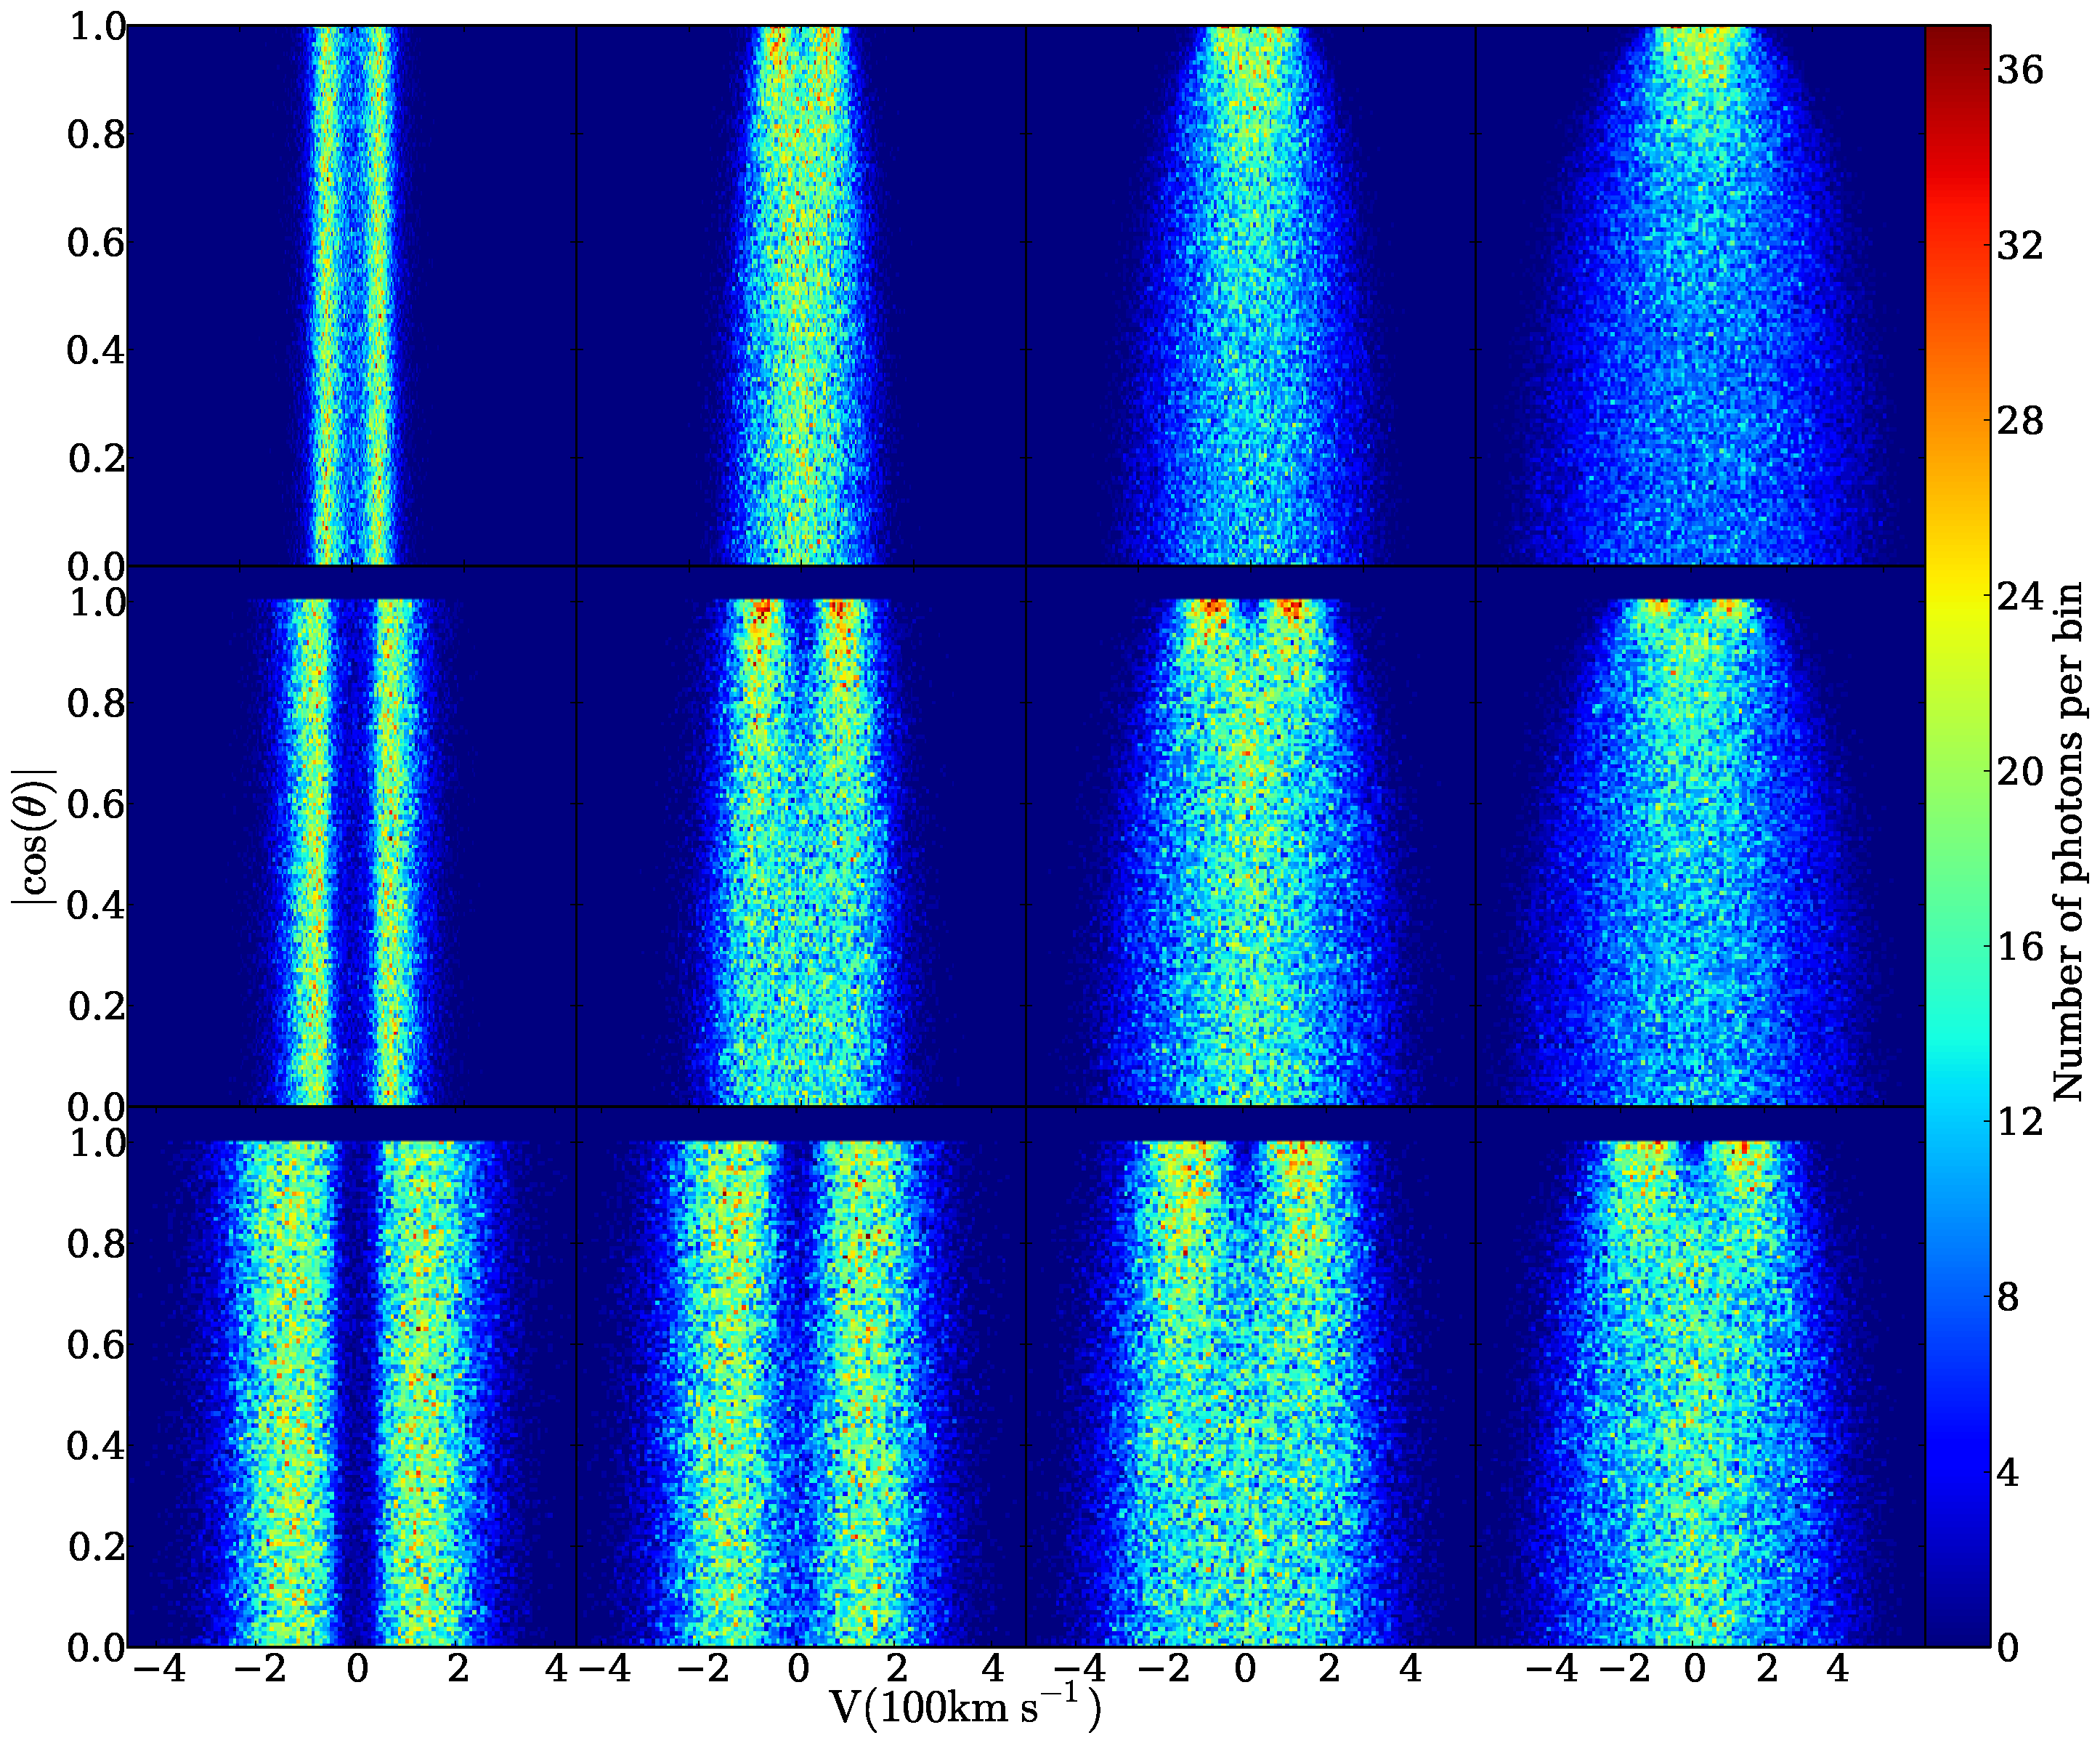
\includegraphics[width=0.95\textwidth]{Figures/f2.pdf}
\end{center}
\caption{
2D histogram showing the number of photons that escape with frequency
$x$ forming an angle $\theta$ (parametrized as $|\cos\theta|$) with the
rotation axis.
The rotational velocity ($0,100,200,300$\kms) increases from left to
right and the optical depth ($10^5$, $10^6$, $10^7$) from top to
bottom.
The \ly photons are initialized at the center of the sphere.
Two main results can be read from this figure.
First, the line morphology depends on the viewing angle.
Second, the line can become single peaked for high rotational
velocities.
\label{fig:CentralSpec} }
\end{figure*}
\begin{figure*}
\begin{center}
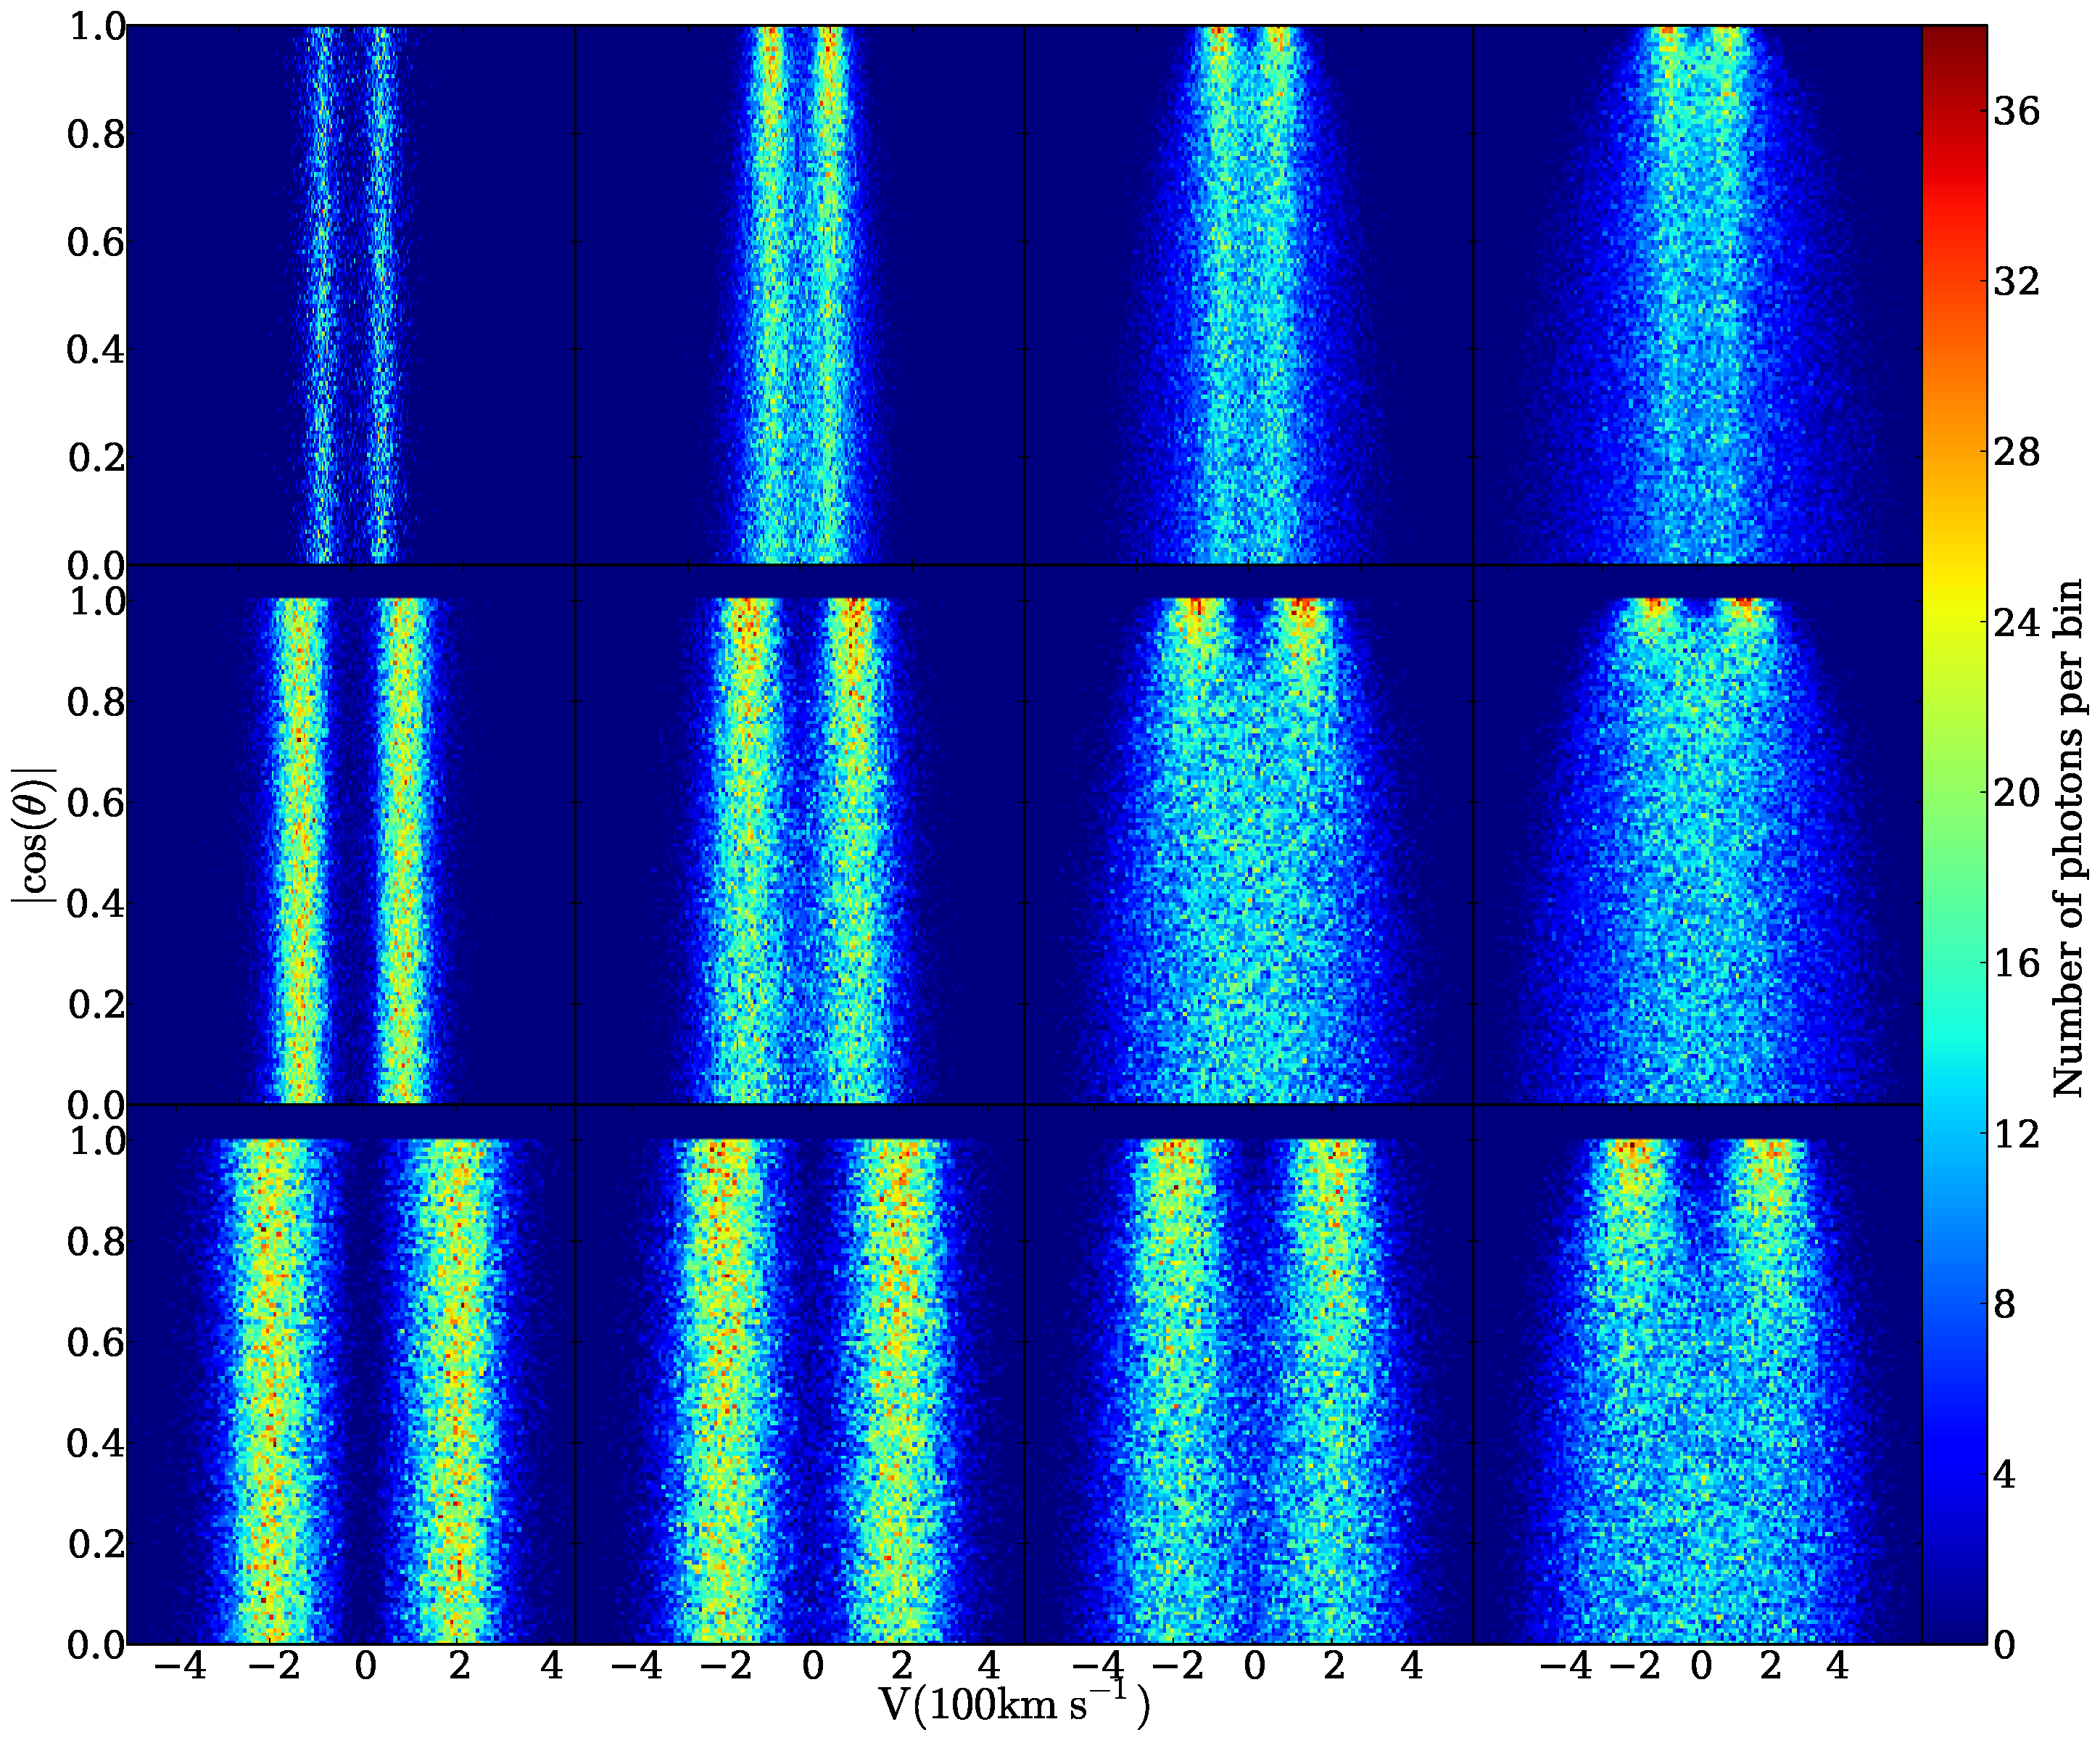
\includegraphics[width=0.95\textwidth]{Figures/f3.pdf}
\end{center}
\caption{Same as Fig. \ref{fig:CentralSpec} for \ly photons
initialized homogeneously throughout the sphere.
\label{fig:HomSpec}}
\end{figure*}
\begin{figure*}
\begin{center}
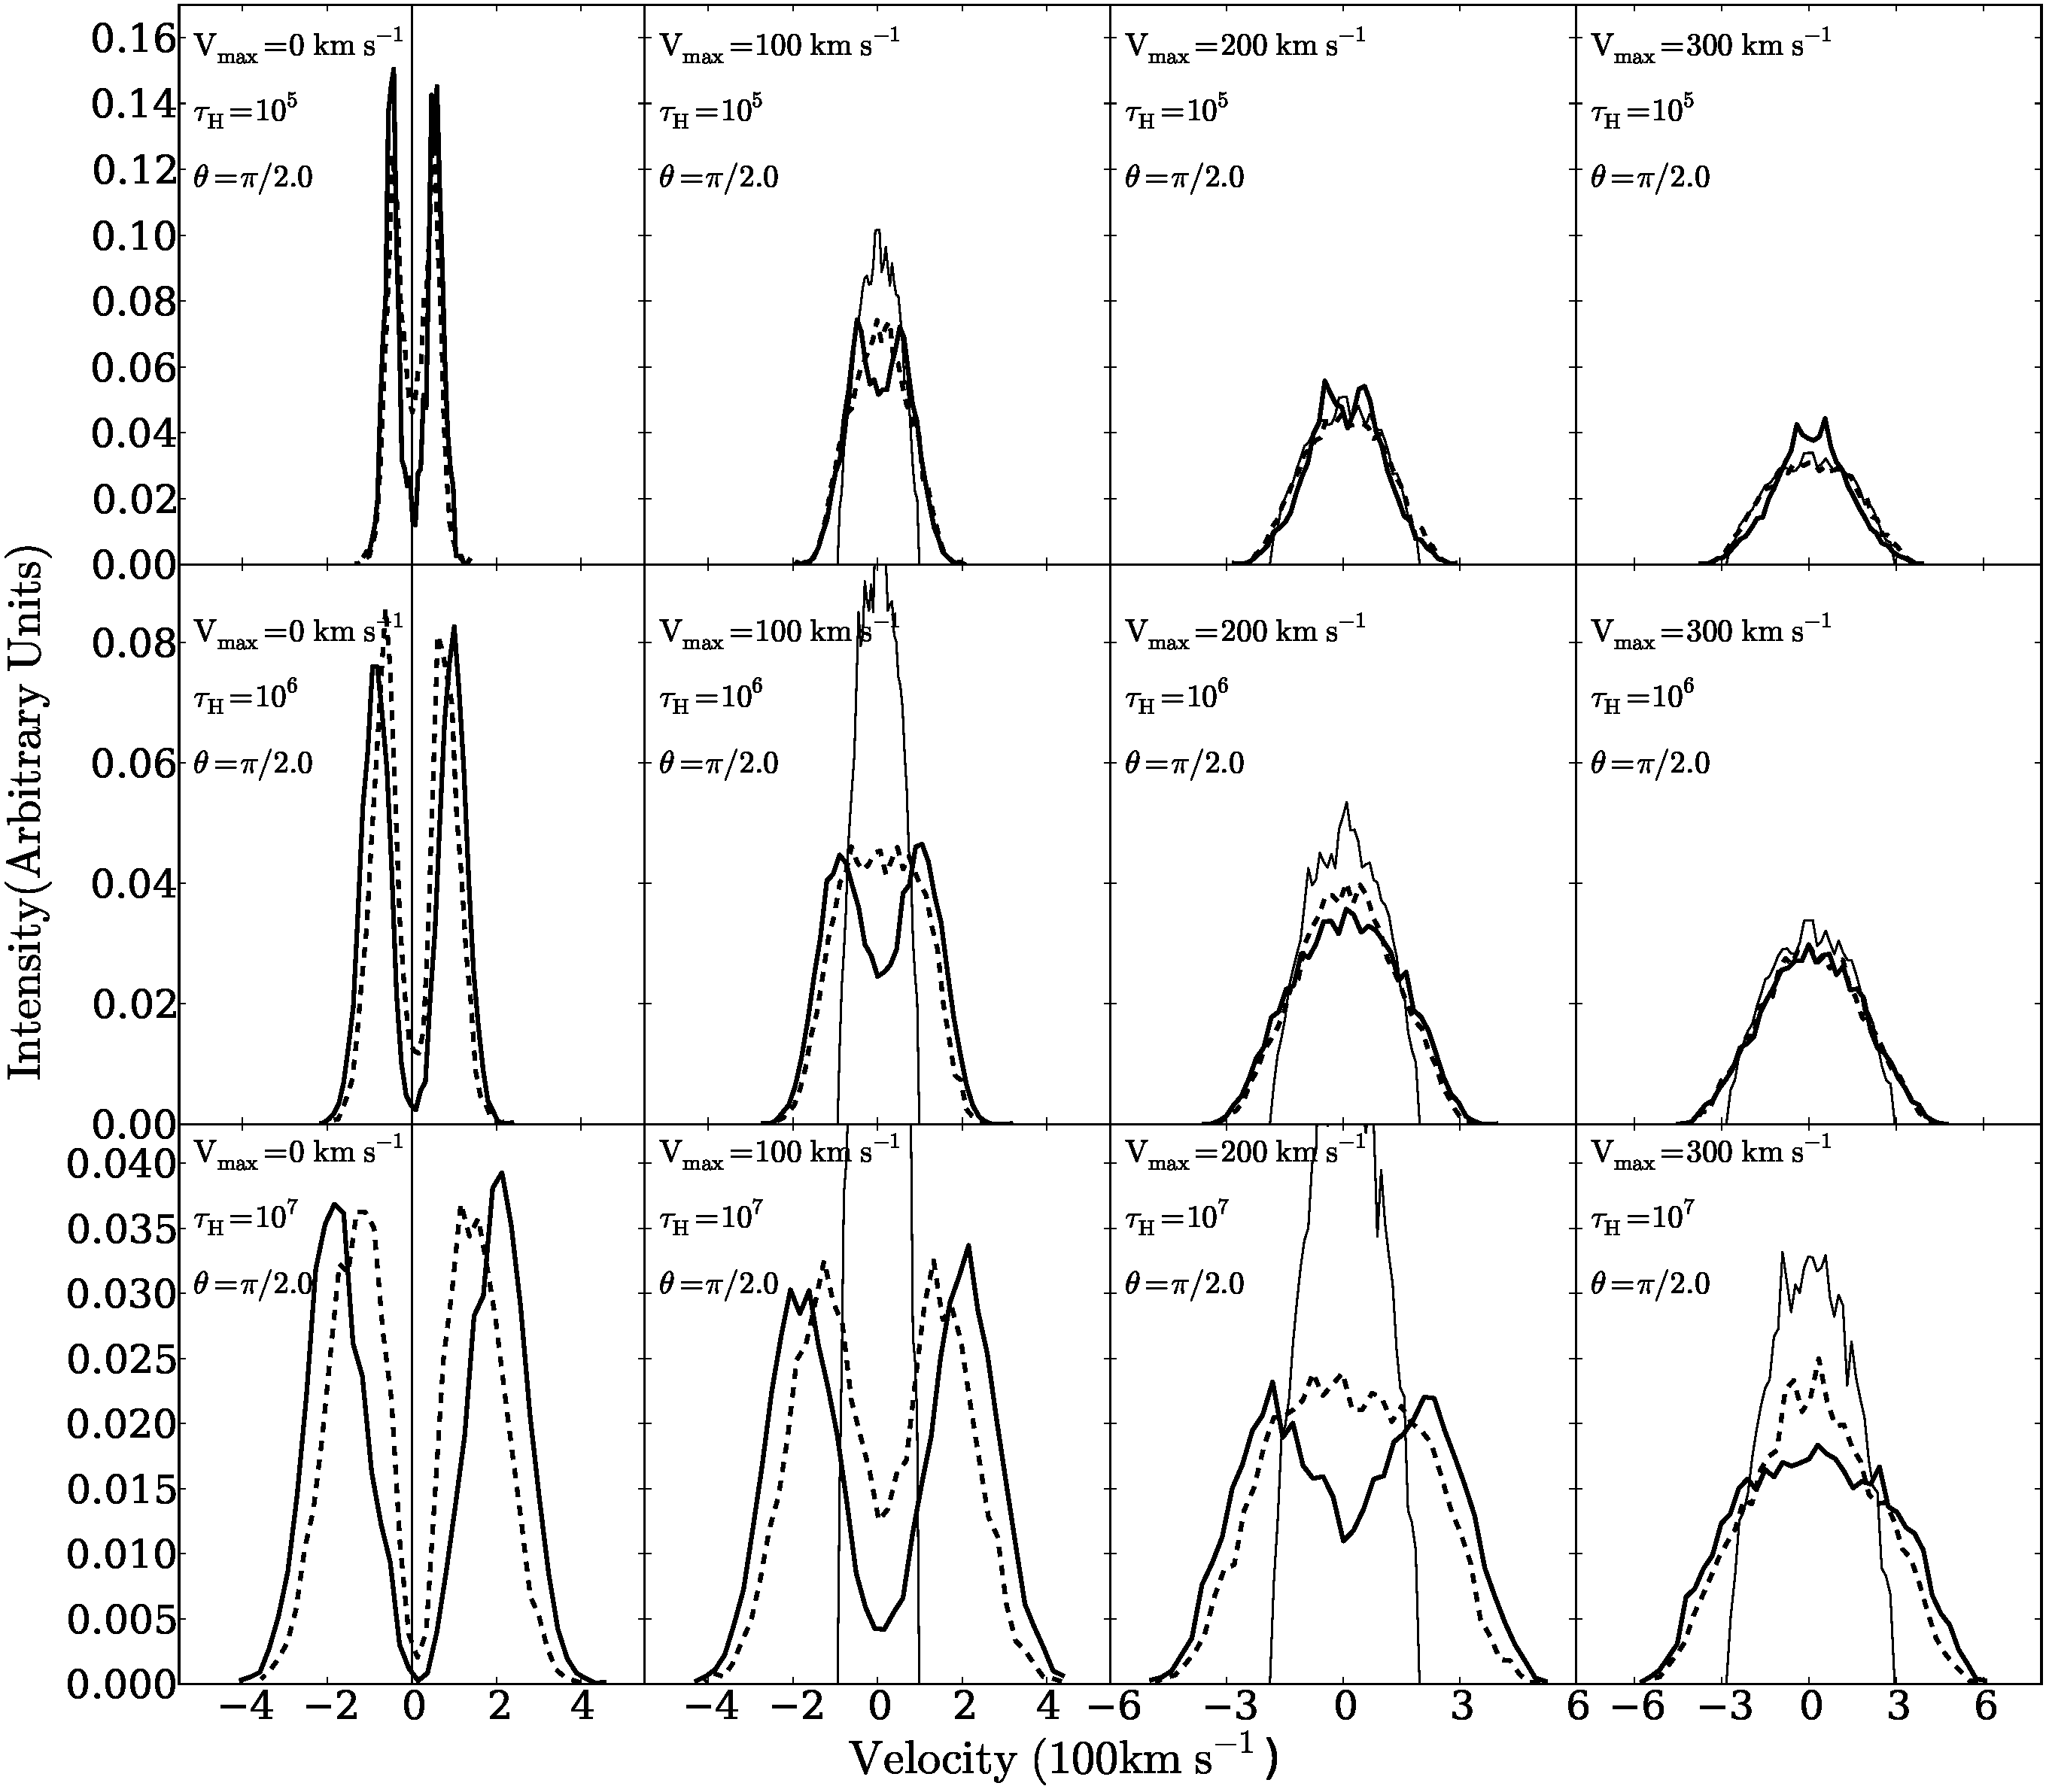
\includegraphics[width=0.95\textwidth]{Figures/f4.pdf}
\end{center}
\caption{Shape of the \ly line for different maximum rotational
velocities for a LoS perpendicular to the rotation axis
($|\mu|\sim 0$). The continuous (dashed) line represents the central
(homogeneous) source distributions. The continuous thin line
represents the intrinsic homogeneous spectrum. The panels follow the same
distribution as in Fig.s \ref{fig:CentralSpec} and \ref{fig:HomSpec}.
\label{fig:differentvelocities}}
\end{figure*}
\begin{figure*}
\begin{center}
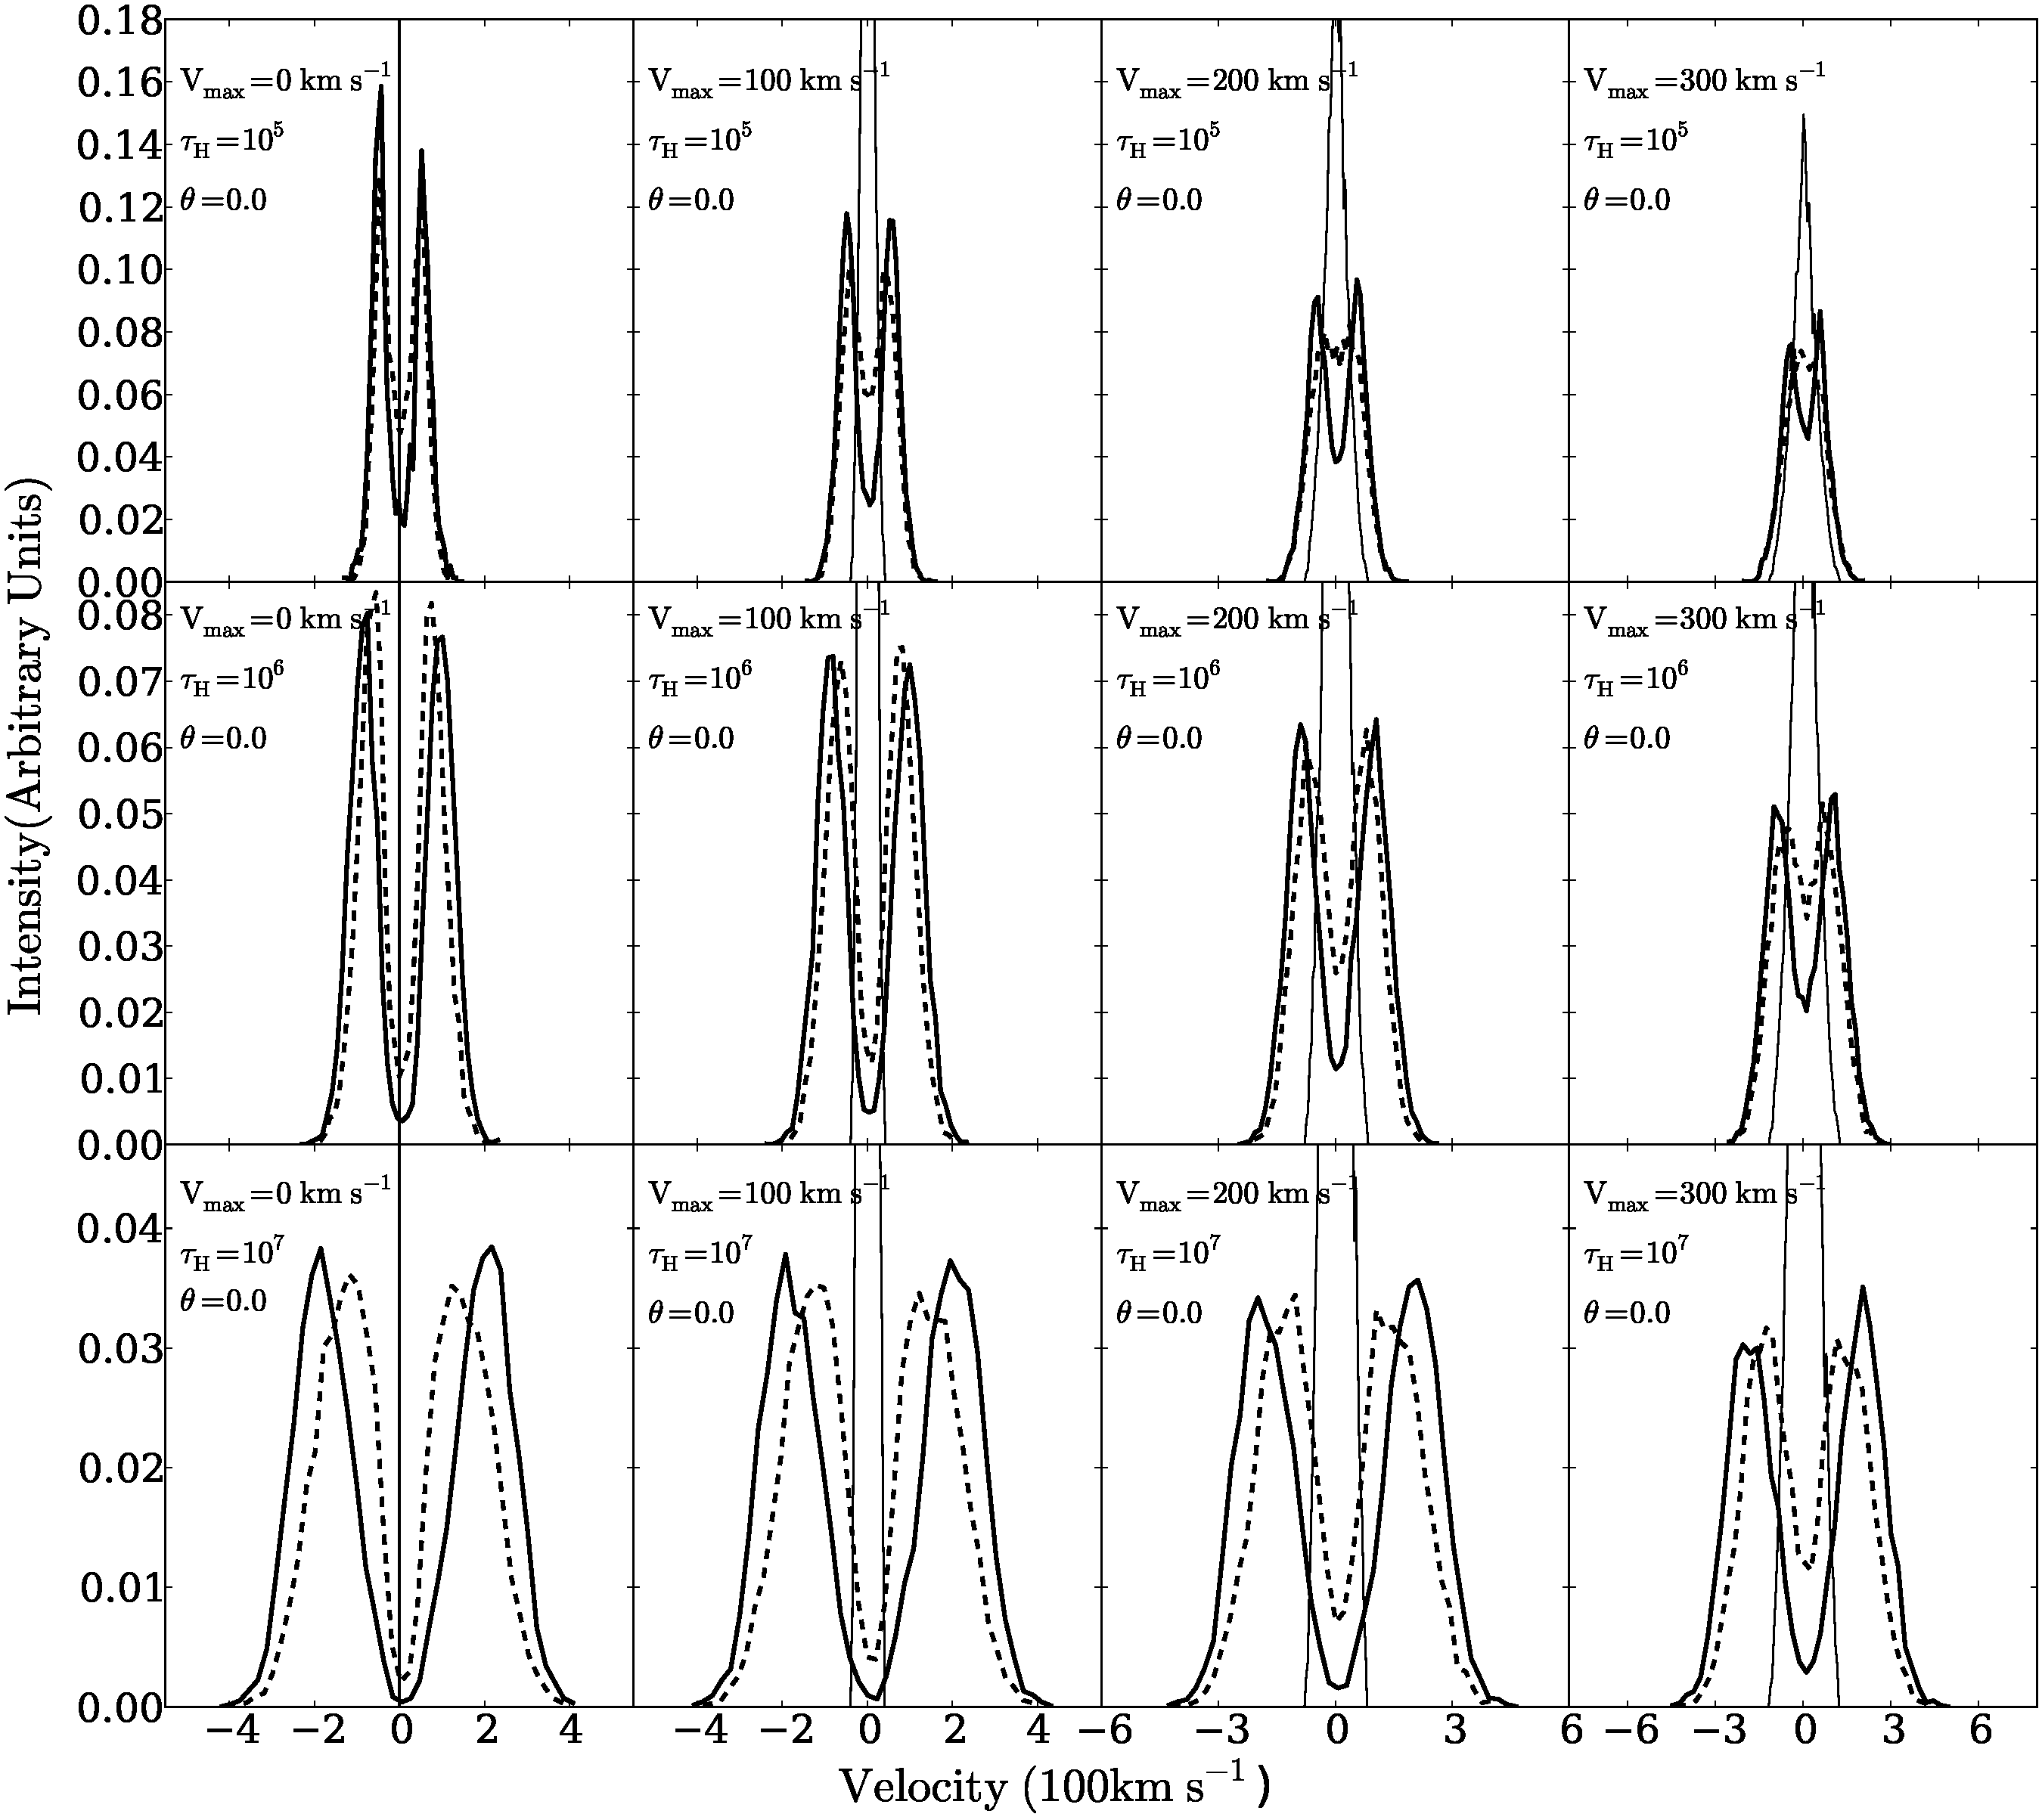
\includegraphics[width=0.95\textwidth]{Figures/f4-2.pdf}
\end{center}
\caption{Shape of the \ly line for different maximum rotational
velocities for a LoS perpendicular to the rotation axis
($|\mu|\sim 1$). The continuous (dashed) line represents the central
(homogeneous) source distributions. The continuous thin line
represent the intrinsic homogeneous spectrum. The panels follow the same
distribution as in Fig.s \ref{fig:CentralSpec} and \ref{fig:HomSpec}.
\label{fig:differentvelocities2}}
\end{figure*}
\subsection{Brief Description of the Radiative Transfer Codes}
Here we briefly describe the relevant characteristics of the two
radiative transfer codes we have used.
For a detailed description we refer the reader to the original papers
\cite{CLARA} and \cite{DijkstraKramer}.
The codes follow the individual scatterings of \ly photons as they
travel through a 3D distribution of neutral Hydrogen.
The frequency of the photon (in the laboratory frame) and
its direction of propagation change at every scattering.
This change in frequency is due to the peculiar velocities of the
Hydrogen absorbing and re-emitting the photon.
Once the photons escape the gas distribution we store their direction of
propagation and frequency at their last scattering.
The initialization process for the \ly photons specifies its
position, frequency and direction of propagation.
We select the initial frequency to be exactly the \ly rest-frame
frequency in the gas reference frame and the direction of propagation
to be random following an flat probability distribution over the sphere.
It means that for photons emitted from the center of the sphere
$x_{\rm in}=0$, while photons emitted at some radii with a peculiar
velocity $\vec{v}$ have initial values $x_{\rm in}$ depending on its direction of
propagation: $x_{\rm in}=\vec{v}\cdot\hat{k}_{\rm in}/v_{\rm th}$.
We do not include the effect of turbulent velocities in the
initialization.
We neglect this given that the induced perturbation should be on the
close to the thermal velocity, $12.8$\kms, which is one order of
magnitude smaller than the velocity widths ($100$-$500$\kms) in the
static case.
If dust is present, the photon can interact either with a Hydrogen
atom or dust grain.
In the case of a dust interaction the photon can be either absorbed or
scattered.
This probability is encoded in the dust albedo, $A$, which we chose
to be $1/2$.
In order to obtain accurate values for the escape fraction of
photons in the presence of dust, we do not use any accelerating
mechanism in the radiative transfer.
The codes treat the gas as homogeneous in density and temperature.
This implies that the gas is completely defined by its geometry
(i.e. sphere or slab), temperature $T$, Hydrogen optical depth
$\tau_{\rm H}$, dust optical depth $\tau_{\rm a}$ and the bulk
velocity field $\vec{v}$.
\subsection{Grid of Simulated Galaxies}
\label{sec:models}
In the Monte Carlo calculations we follow the propagation of $N_{\gamma}=10^5$
numerical photons through different spherical galaxies.
For each galaxy we vary at least one of the following parameters: the maximum
rotational velocity $V_{\rm max}$, the hydrogen optical depth $\tau_{H}$,
the dust optical depth $\tau_{a}$ and the initial distribution of photons
with respect to the gas.
In total there are $48$ different models combining all the possible
different variations in the input parameters.
Table \ref{table:models} lists the different parameters we used to
generate the models. The results and trends we report are observed in both
Monte Carlo codes.
\begin{table}
\begin{center}
\begin{tabular}{llc}\hline\hline
Physical Parameter (units) & Symbol & Values\\\hline
Velocity (\kms) & $V_{\rm max}$&$0,\ \ 100,\ 200,\ 300$\\
Hydrogen Optical Depth & $\tau_{H} $ & $10^{5},\ 10^{6},\ 10^{7}$\\
Dust Optical Depth & $\tau_{a}$ & $0$,$1$\\
Photons Distributions & & Central, Homogeneous\\\hline\hline
\end{tabular}
\caption{
Summary of Physical Parameters of our Monte Carlo Simulations.}
\label{table:models}
\end{center}
\end{table}
\section{Results}
\label{sec:results}
The main results of this paper are summarized in Fig.
\ref{fig:CentralSpec} and \ref{fig:HomSpec}.
They show 2D histograms of the escape frequency $x$ and outgoing angle
$\theta$ parametrized by $|\mu|$.
Taking into account only photons photons around a value
of $|\mu|$ gives us the emission detected by an observer located at an
angle $\theta$ with respect to the rotation axis.
We have verified that the solutions are indeed symmetric with respect
to $\mu=0$. We have also verified that the total flux is the same for all $\mu$.
From these figures we can see that the line properties change with
rotational velocity and depend on the viewing angle $\theta$.
In the next subsections we quantify the morphology changes with with
velocity, optical depth and viewing angle.
We characterize the line morphology by its total intensity, the full
width at half maximum, (FWHM) and the location of the peak maxima.
In order to interpret the
morphological changes in the line we also report the median number of
scatter for each \ly photon in the simulation.
For the models where dust is included we measure the escape fraction
as a function of rotational velocity and viewing angle.
\subsection{Line Morphology}
\label{sec:angles}
The first column in both Fig. \ref{fig:CentralSpec} and
\ref{fig:HomSpec} shows that for the static sphere the line properties
are independent of $|\mu|$, as it is expected due
to the spherical symmetry.
However, for increasing rotational velocities, at a fixed optical
depth, there are clear signs that this symmetry is broken.
If the viewing angle is aligned with the rotation axis, $|\mu|\sim
1$, the \ly line keeps a double peak with minor
changes in the morphology as the rotational velocity increases.
However, for a line of sight perpendicular to the rotation axis,
$|\mu|\sim 0$, the impact of rotation is larger.
The double peak readily transforms into a single peak.
This is clear in Fig. \ref{fig:differentvelocities} and in Fig.
\ref{fig:differentvelocities2} where we
present the different line morphologies for $|\mu|\sim 0$ and
$|\mu|\sim 1 $ for the
homogeneous and central configurations.
The panels have the same distribution as Fig. \ref{fig:CentralSpec}
and \ref{fig:HomSpec}.
There are three clear effects on the line morphology as the rotational
velocity increases.
First, the line broadens; second, the double peaks reduce their intensity; and
third, the intensity at the line centre rises.
The last two effects are combined to give the impression that the double
peaks are merged into a single one at high rotational velocities.
\subsection{Integrated Line Intensity}
\label{sec:intlineint}
\begin{figure}
\begin{center}
\includegraphics[width=0.4\textwidth]{Figures/f5.pdf}
\end{center}
\caption{Integrated flux distribution as a function of the
viewing angle as parametrized by $\mu$. Continuous (dashed)
correspond to central (homogeneous) source distribution.
The models correspond to an optical depth of $\tau_{\rm
H}=10^5$ and rotational velocities of $100$\kms, $200$\kms and
$300$\kms. The distributions are flat in the range of models probed
in this paper, meaning that the integrated flux for all viewing
angles is the same.
\label{fig:muhisto}}
\end{figure}
We now consider possible variations in the integrated flux with
respect to the viewing angle $\theta$.
To this end we define the normalized flux seen by an observer at an
angle $\mu$ by:
\begin{equation}
F(\mu) = \frac{2\Delta N}{N\Delta \mu},
\end{equation}
%
where $\mu=\cos\theta$, $N$ is the total number of outgoing photons,
$\Delta N$ is the number of photons in an angular bin $\Delta
\theta$. This definition satisfies the condition
$\int_{-1}^{1}F(\mu)d\mu/2=1$. In the case of perfect spherical
symmetry one expects a flat distribution with $F(\mu)=1$.
Fig. \ref{fig:muhisto} shows the results for a selection of models
with $\tau_{\rm H}=10^{5}$, different rotational velocities and the two
types of source distributions. This shows that $F(\mu)$ is consistent with being flat, apart
from some statistical fluctuations on the order of 2\%.
This is a remarkable result: while the rotation axis defines preferential direction, the
integrated flux is the same for all viewing angles in the range of parameters explored in this paper. This can be understood from the fact that
{\it radiative transfer inside a sphere that undergoes solid-body
rotation proceeds identical as inside a static sphere}: we can draw
a line between any two atoms within the rotating cloud, and their
relative velocity along this line is zero (apart from the relative
velocity as a result of random thermal motion), irrespective of the
rotation velocity of the cloud. This relative velocity is what is
relevant for the radiative transfer\footnote{This point can be further
illustrated by considering the path of individual photons: let a
photon be emitted at line center ($x=0$), in some random direction
${\bf k}$, propagate a distance that corresponds to $\tau_0=1$,
scatter fully coherently (i.e. $x=0$ after scattering in the gas
frame) by 90$^{\circ}$, and again propagate a distance that
corresponds to $\tau_0=1$. The position where the photon scatters
next does {\it not} depend on the rotation of the cloud, nor on
${\bf k}$.}
\subsection{Full Width at Half Maximum}
\label{sec:widthpeak}
\begin{figure*}
\begin{center}
\includegraphics[width=0.95\textwidth]{Figures/f6.pdf}
\end{center}
\caption{FWHM for the non-dusty models as a function of the viewing
angle parametrized by $|\cos\theta|$. Continuous (dashed) lines correspond
to central (homogeneous) source distributions. The general trend is
of an decreasing line width as the line of sight becomes parallel to the
rotation axis.
\label{fig:widthvsmu}}
\end{figure*}
\begin{figure*}
\begin{center}
\includegraphics[width=0.95\textwidth]{Figures/f7.pdf}
\end{center}
\caption{FWHM for the non-dusty models as a function of
rotational velocity $V_{\rm max}$ for observers located
perpendicular to the rotation axis.
The left panel shows the results in velocity units while the right
panel normalizes the data by the FWHM in the static case.
Continuous (dashed) lines correspond to central (homogeneous)
source distributions.
The straight lines represent the fit to the data using the
expression in Eq. (\ref{eq:fwhm}).
\label{fig:widthsvsvelocity}}
\end{figure*}
We use the full width at half maximum (FWHM) to quantify the line
broadening.
We measure this width from the line intensity histogram by finding the
values of the velocities at half maximum intensity.
We use lineal interpolation between histogram points to get a value
more precise than the bin size used to construct the histogram.
Fig. \ref{fig:widthvsmu} shows the FWHM for all models as a function
of the viewing angle.
The FWHM increases for decreasing values of $\mu$ (movement from the
poles to the equator) and increasing values of $V_{\rm max}$.
In Fig.
\ref{fig:widthsvsvelocity} we fix $|\mu|<0.1$, i.e. viewing angle
perpendicular to the rotation axis, to plot the FWHM as a function of
rotational velocity.
We parametrize the dependency of the line width with $V_{\rm max}$ as
%
\begin{equation}
{\rm FWHM}^2 = {\rm FWHM}_{0}^2 + V_{\rm max}^2/\lambda^2,
\label{eq:fwhm}
\end{equation}
%
where FWHM$_{0}$ is the velocity width in the static case and $\lambda$
is a positive scalar to be determined as a fit to the data.
With this test we want to know to what extent the new velocity width can be
expressed as a quadratic sum of the two relevant velocities in the
problem.
All the models fall into a single family of lines in the plane shown
in the right panel of Fig. \ref{fig:widthsvsvelocity}, justifying
the choice of our parametrization.
We fit simultaneously all the points in two separate groups, central
and homogeneous sources.
We find that these values are $\lambda_{\rm c} = 0.83 \pm 0.06$ and
$\lambda_{\rm h}= 0.82\pm 0.05$ respectively.
\subsection{Line Maxima}
\label{sec:maxima}
\begin{figure*}
\begin{center}
\includegraphics[width=0.95\textwidth]{Figures/f8.pdf}
\end{center}
\caption{Position of the line maxima as a function of maximum
rotational velocity $V_{\rm max}$. Continuous (dashed) lines
correspond to central (homogeneous) source distributions. A value
of $x_{\rm max}=0$ indicates that line becomes single
peaked. \label{fig:maximumvsvelocity}}
\end{figure*}
We measure the peak maxima position, $x_m$, to quantify the transition from
double into single peak profiles.
In Fig. \ref{fig:maximumvsvelocity} we show the dependence of $x_m$ with
the viewing angle parametrized by $|\cos\theta|$ for different
rotational velocities.
There are two interesting features that deserve attention.
First, for a viewing angle parallel to the rotational axis ($\mu\sim
1.0$) the maxima of all models with the same kind of source
initialization are similar regardless of the rotational velocity.
Second, at a viewing angle perpendicular to the rotation axis ($\mu\sim 0.0$) a
large fraction of models become single peaked.
This feature appears more frequently for homogeneously distributed
sources if all the other parameters are equal.
\subsection{Dusty Clouds: Escape Fraction}
\label{sec:escapefraction}
\begin{table}
\begin{center}
\begin{tabular}{c cccccc}
\hline \hline
Source & $\tau_{H}$ & & $\ V_{\rm max}$& & \\
Distribution& & & (\kms) & & \\
& & 0 & 100 &200 & 300\\ \hline
Homogeneous & $10^{5}$& 0.263 & 0.263 & 0.263 & 0.263 \\
& $10^{6}$ & 0.291 & 0.292 & 0.293 & 0.293 \\
&$10^{7}$ & 0.228 & 0.228 & 0.228 & 0.228 \\
Central & $10^{5}$ & 0.096 & 0.096 & 0.096 & 0.096 \\
&$10^{6}$ & 0.066 & 0.066 & 0.066 & 0.066 \\
&$10^{7}$ & 0.015 & 0.016 & 0.016 & 0.015 \\
\hline
\end{tabular}
\caption{
Escape fraction values for all dusty models. }
\label{table:escape}
\end{center}
\end{table}
We now estimate the escape fraction $f_{\rm esc}$ for the dusty
models. The main result is that we do not find any significant dependence
with either the viewing angle nor the rotational velocity. This is consistent with our finding in \S~\ref{sec:intlineint}, that radiative transfer inside the cloud does not depend on its rotational velocity. For completeness we list in Table \ref{table:escape} the escape
fraction for all models.
We now put these results in the context of the analytic solution for
the infinite slab\citep{Neufeld90}.
In Neufeld's set-up the analytic solution depends
uniquely on the product $(a\tau_{\rm H})^{1/3}\tau_{A}$ where
$\tau_{A} = (1 - A)\tau_{a}$, valid only in the limit $a\tau_{\rm
H}\gg 1$.
At fixed values of $\tau_{a}$ the escape fraction monotonically
decreases with increasing values of $\tau_{\rm H}$.
This expectation holds for the central sources.
But in the case of homogeneous sources the escape fraction increases
slightly from $\tau_{\rm H}=10^5$ to $\tau_{\rm H}=10^{6}$
The naive interpretation of the analytic solution does not seem to
hold for photons emitted far from the sphere's center.
We suggest that increasing $\tau_{\rm H}$ from $10^{5}$ to $10^{6}$ causes a
transition from the 'optically thick' to the 'extremely optically
thick' regime for a noticeable fraction of the photons in the
homogeneous source distribution.
In the optically thick regime, \ly photons can escape in
'single flight' which corresponds to a scenario in which the
photon resonantly scatters $10^4-10^5$ times until it is scattered
into the wing of the line ($x\sim 3-4$).
At these frequencies the medium is optically thin, and the photons can
escape efficiently in a single flight.
In contrast, in an extremely optically thick medium \ly
photons escape in a `single excursion' \citep{Adams72}.
Here, photons that are scattered into the wing of the line escape from
the medium in a sequence of wing scattering events.
In both cases, \ly photons resonantly scatter $10^4$-$10^5$ times.
Because we keep our clouds the same size, the mean free path of Lya
photons that scatter resonantly is 10 times larger for the case
$\tau_{\rm H}=10^5$ than for $\tau_{\rm H}=10^6$.
If we compute the average distance $D$ travelled by \ly
photons through a medium of size $R$ as a function of line center
optical depth $\tau_{\rm H}$, then we find that during the transition
from optically thick to extremely optically thick the mean traversed
distance $D$ actually decreases slightly.
This decrease is unique to this transition region, and $D$ generally
increases with $\tau_{\rm H}$ at other values of $\tau_{\rm H}$.
\subsection{Average Number of Scatterings}
\label{sec:scatterings}
\begin{figure*}
\begin{center}
\includegraphics[width=0.45\textwidth]{Figures/f12.pdf}
\includegraphics[width=0.45\textwidth]{Figures/f13.pdf}
\end{center}
\caption{2D histogram of the logarithm of the average number of scatterings as function of $\mu$ (left) and the maximum rotational velocity $V_{\rm
max}$ (right). The left panel shows the behaviour for $\tau=10^{5}$ and
$V_{max}=300$\kms as a function of $\left|\cos\theta\right|$, the color indicates the number of photons per bin. In the
right panel the continous (dashed) lines represent the results for
the central (homogeneous) model. The independence of $N_{\rm scatt}$ with $\mu$ and $V_{\rm max}$ is
present in all models.
\label{fig:Nscatt} }
\end{figure*}
The number of scatterings affects the escape frequency of a \ly
photon. Studying this quantity further illustrates the independence of
the integrated flux and the escape fraction on rotational velocity.
In Fig. \ref{fig:Nscatt} we show the average number of scatterings
$\langle N_{\rm scatt}\rangle$ as a function of the cosinus of the
outgoing angle $|\cos\theta|$ and the rotational velocity
$V_{\rm max}$.
From the right panel observe that the number of scatterings and the
outgoing angle are independent.
This plot corresponds to the specific case of the central model with
$\tau=10^5$ and $V_{\rm max}=300$\kms, but we have verified that this
holds for all models.
The right panel of Fig. \ref{fig:Nscatt} shows how the average
number of scatterings is also independent from the rotational
velocity.
The lower number of average scatterings in the homogeneous source
distribution is due to a purely geometrical effect.
Photons emitted close to the surface go through less scatterings
before escaping.
In static configurations it is expected that the optical depth correlates number of
scatterings.
This has been precisely quantified in the case of static infinite
slab.
In that model for centrally emitted sources the average number of
scatterings depends only on the optical depth $\langle N_{\rm
scatt}\rangle=1.612\tau_{\rm H}$ \citep{Adams72,Harrington73}, for
homogeneously distributed sources $\langle N_{\rm
scatt}\rangle=1.16\tau_{\rm H}$ \citep{Harrington73}.
In our case we find that for the central model the number of
scatterings is proportional to the optical depth, with $\langle N_{\rm
scatt}\rangle= (1.50, 1.00, 0.92)\tau_{\rm H}$ for optical depth
values of $\tau_{\rm H} = (10^{5}, 10^{6}, 10^{7})$ respectively.
For the homogeneous sources we find that $\langle N_{\rm
scatt}\rangle= (0.99, 0.59, 0.51)\tau_{\rm H}$.
\section{Discussion}
\label{sec:discussion}
\subsection{Towards an analytical description}
There is a key result of our simulations that allows us to build an
analytical description for the outgoing spectra.
It is the independence of the following three quantities with the rotational
velocity and the viewing angle: integrated flux, average number of
scatterings and escape fraction.
As we explained in \S~\ref{sec:intlineint}, the best way to understand this is that radiative transfer inside a sphere that undergoes solid-body rotation
proceeds identical to that inside a non-rotating sphere. While scattering events off atoms within the rotating cloud impart
Doppler boosts on the Ly$\alpha$ photon, these Doppler boost are only
there in the lab-frame. Therefore, in the frame of the rotating gas cloud all atoms are
stationary with respect to each other and the scattering process
proceeds identical as in the static case (also see \S~\ref{sec:intlineint} for an additional more quantitative explanation).
This result allows us to analytically estimate the spectrum emerging from a rotating cloud:
The spectrum of \lya photons emerging from a rotating gas cloud is identical as for the static case in a frame that is co-rotating
with the cloud. However, the surface of cloud now moves in the lab-frame.
Each surface-element on the rotating cloud now has a bulk
velocity with respect to a distant observer. In order to compute the
spectrum one can integrate over all the surface elements in the
sphere with their corresponding shift in velocity and an additional
weight by the surface intensity.
Fig~\ref{fig:comparison} shows some examples of analytic versus full MC
spectra using this approach (the implementation details are in the Appendix).
The left panel shows the results for different rotational velocities
in the case of $\tau_{H}=10^7$ and an observer located perpendicular
to the axis of rotation ($i=0$ in the scheme of Fig~\ref{fig:scheme}
in the Appendix). The right panel shows the results for different viewing angles in the
case of $\tau_{H}=10^7$ and a rotational velocity of $V_{\rm
max}=300$\kms.
The two methods clearly give good agreement, though not perfect. In particular, the left panel shows that the MC gives rise to a spectrum that is
slightly more concentrated towards the line centre. As we explain in Appendix~\ref{sec:app}, we do not expect perfect agreement, because this requires an analytic solution for the spectrum of Ly$\alpha$ photons emerging from a static, optically extremely thick cloud {\it as a function of the angle at which they escape from the sphere}. This solution does not exist in the literature. It is possible to get better agreement my modifying the surface brightness profile.
In any case, the analytic calculation closely captures the results
obtained from the full calculations from the MC simulations.
As such, they are extremely useful and provide us with a quick tool to
verify our calculations at the first order level.
\begin{figure*}
\begin{center}
\includegraphics[width=0.49\textwidth]{Figures/fig10a.pdf}
\includegraphics[width=0.49\textwidth]{Figures/fig10b.pdf}
\end{center}
\caption{
Comparison of the Monte Carlo results against the analytic
solution. The left panel explores the results of different velocities.
The right panel presents the results for two different observers:
paralel and perpendicular to the rotational axis, $\mu=1$ and $\mu=0$
respectively.
\label{fig:comparison} }
\end{figure*}
\subsection{Impact on the interpretation of simulated and
observational data}
We now compare our findings to other computational results and discuss
its possible implications for the interpretation of observational data.
{\bf Escape at Line Center.} Our models have shown that rotation
enhances the flux density at line center (see Fig. \ref{fig:differentvelocities}). It has
recently been proposed that galaxies with Lya spectral lines that
contain flux at line center may be `leaking' ionizing (LyC) photons
\citep{Behrens2014,2014arXiv1404.2958V}. The main reason for this possible
connection is that the escape of ionizing (LyC) photons requires
$N_{\rm HI} < 10^{17} $cm$^{-2}$. The same low column densities facilitate the escape of
\ly photons at (or close to) line center. Our work suggests that
rotation may provide an alternative explanation.
{\bf Single peaked lines}. The presence of single peaked profiles has
been associated to inflow/outflow dynamics
\citep{Verhamme06,DijkstraKramer}.
Gas bulk rotation can also be considered as a probable origin for that
behaviour, provided that the observed single peak is highly
symmetric.
Similarly, in the case of double peaked lines with a high
level of flux at the line center, rotation also deserves to be
considered in the pool of possible bulk flows responsible for that feature,
specially if the two peaks have similar intensities.
{\bf Systemic velocities}. There are observational measurements for the
velocity shift between the \ly and other emission lines. In our study
we find that the position of the peak maxima can suddenly change with
rotation and viewing angle. Namely the line can become single peaked
for high rotational velocities and viewing angles perpendicular to the
rotation axis.
{\bf Galaxy simulations with gas rotation}. \cite{Verhamme12} studied \ly
line emission in two high resolution simulations of individual
galaxies.
The main purpose of their study was to assess the impact of two
different ISM prescriptions.
However, each simulated galaxy had a disc structure with a clear rotation pattern in
the ISM and inflowing gas from the circum-galactic region.
The configuration had an axial symmetry and they reported a strong dependence of both
the escape fraction and the total line intensity as a function of the
$\theta$ angle.
From our study, none of these two quantities has a dependence either
on the inclination angle or the rotational velocity.
We suggest that he effect reported by \cite{Verhamme12} is
consistent with being a consequence of the different hydrogen optical
depth for different viewing angles and not as an effect of the bulk
rotation.
{\bf Zero impact on the \ly escape fraction}. Study of
high redshift LAEs in numerical simulation often requires the
estimation of the \ly escape fraction in order to compare their
results against observations
\citep{CLARA,Dayal2012,Forero12,Orsi12,Garel2012}. Most of these
models estimate the escape fraction from the column density of dust and
neutral Hydrogen. The results of our simulation indicate that the
rotational velocity does not induce additional uncertainties in those
estimates.
\section{Conclusions}
\label{sec:conclusions}
In this paper we quantified for the first time in the literature the effects
of gas bulk rotation in the morphology of the \ly emission line in
star forming galaxies.
Our results are based on the study of an homogeneous sphere
of gas with solid body rotation.
We explore a range of models by varying the rotational speed, hydrogen
optical depth, dust optical depth and initial distribution of \ly
photons with respect to the gas density.
As a cross-validation, we obtained our results from two independently
developed Monte-Carlo radiative transfer codes.
Two conclusions stand out from our study.
First, rotation clearly impacts the \ly line morphology; the width and
the relative intensity of the center of the line and its peaks are
affected.
Second, rotation introduces an anisotropy for different viewing
angles.
For viewing angles close to the poles the line is double peaked and it
makes a transition to a single peaked line for high rotational
velocities and viewing angles along the equator.
This trend is clearer for spheres with homogeneously distributed
radiation sources than it is for central sources.
Remarkably, we find three quantities that are invariant with respect
to the viewing angle and the rotational velocity: the integrated flux,
the escape fraction and the average number of scatterings.
These results helped us to construct the outgoing spectra of a
rotating sphere as a superposition of spectra coming from a static
configuration. This description is useful to describe the main
quantitative features of the Monte Carlo simulations.
Quantitatively, the main results of our study are summarized as
follows.
\begin{itemize}
\item In all of our models, rotation induces changes in the line morphology
for different values of the angle between the rotation
axis and the LoS, $\theta$. The changes are such that for
a viewing angle perpendicular to the
rotation axis, and high rotational velocities the line becomes single peaked.
\item The line width increases with rotational
velocity. For a viewing angle perpendicular to the rotation axis
This change approximately follows the functional form ${\rm FWHM}^2
= {\rm FWHM}_{ 0}^2 + (V_{\rm max}/\lambda)^2$, where FWHM$_{0}$
indicates the line
width for the static case and $\lambda$ is a constant. We have
determined this constant to be $\lambda_{\rm c}=0.83 \pm 0.06$ and
$\lambda_{\rm h}=0.82\pm 0.05$ for the central and homogeneous source
distributions, respectively.
\item At fixed rotational velocity the line width decreases as $|\mu|$
increases, i.e. the smallest value of the line width is observed for
a line of sight parallel to the ration axis.
\item The single peaked line emerges at viewing angles $\mu\sim 1$ for
when the rotational velocity is close to than half the FWHM$_0$.
\end{itemize}
Comparing our results with recent observed LAEs we find that
morphological features such as high central line flux, single peak
profiles could be explained by gas bulk rotation present in these
LAEs.
The definitive and clear impact of rotation on the \ly morphology
suggests that this is an effect that should be taken into account at
the moment of interpreting high resolution spectroscopic data. In
particular it is relevant to consider the joint effect of rotation the
and ubiquitous outflows (M.C. Remolina-Gutierrez et al., in prep.)
because rotation can lead to enhanced escape of \ly at line center, which
has also been associated with escape of ionizing (LyC) photons
\citep{Behrens2014,2014arXiv1404.2958V}
\section*{Acknowledgments}
JNGC acknowledges financial support from Universidad de los
Andes.
JEFR acknowledges financial support from Vicerrectoria de
Investigaciones at Universidad de los Andes through a FAPA grant.
We thank the International Summer School on AstroComputing
2012 organized by the University of California High-Performance
AstroComputing Center (UC-HiPACC) for providing computational
resources where some of the calculations were done.
The data, source code and instructions to
replicate the results of this paper can be found
here {\texttt{https://github.com/jngaravitoc/RotationLyAlpha}}.
Most of our code benefits from the work of the IPython and Matplotlib
communities \citep{IPython,matplotlib}.
We thank the referee for the suggestions that allowed us to greatly
improve and better frame the interpretation of our simulations.
\appendix

\section{Appendix: Analytic Expression for the Ly$\alpha$ Spectrum
emerging from Rotating Cloud}\label{sec:app}




Ly$\alpha$ scattering through an optically thick gas cloud that is
undergoing solid-body rotation (i.e. in which the angular speed around the
rotation axis is identical for each hydrogen atom) proceeds identical
as in a static cloud. In order to compute the spectrum emerging from a rotating cloud, we sum
the spectra emerging from all surface elements of the cloud, weighted by their intensity.
We adopt the geometry shown in Fig~\ref{fig:scheme} to derive an analytic expression of this emerging spectrum,
Note that this geometry differs from the scheme shown in Fig~1 in the main body of
the paper.
%
\begin{figure*}[h]
\centerline{\includegraphics[width=80mm]{Figures/fig11a.pdf}
\includegraphics[width=80mm]{Figures/fig11b.pdf}}
\caption[]{Adopted geometry for evaluating the analytic spectrum.}
\label{fig:scheme}
\end{figure*}
%
The sightline to the observer \& rotation axis define the $x-z$ plane.
The {\it left panel} in Fig~\ref{fig:scheme} shows the view from the $y$-axis.
The observer sits along the $x$ axis.
The rotation axis makes an angle $i$ with respect to the $z$-axis.
We sum up spectra from individual patches by integrating over the
impact parameter $b$, and angle $\phi$.
Each $(b,\phi)$ corresponds to a point on the sphere.
This point has a velocity vector ${\bf v}(b,\phi,i)$, which we denote
with ${\bf v}$ for brevity. The magnitude of ${\bf v}$ is $|{\bf v}|=V_{\rm max}R'/R$. Here $R'=\sqrt{R^2 -s^2}$, in which $s$ denotes the distance of the point $(b,\phi)$ to the plane perpendicular to the rotation axis and through the origin (see the {\it left panel} of Fig~\ref{fig:scheme}). This distance $s$ is given by $s=|-\sin i\sqrt{R^2-b^2}+ b \cos \phi \cos i|$.\\
The spectrum of the flux emerging from the surface at point $(b,\phi)$ is
\begin{displaymath}
J(x,b,\phi,i)=\frac{\sqrt{\pi}}{\sqrt{24}a\tau_0}\Bigg{(}\frac{(x-x_{\rm
b})^2}{1+{\rm cosh}\Big{[}\sqrt{\frac{2\pi^3}{27}}\frac{|(x
-x_{\rm b})^3|}{a\tau_0}\Big{]}}\Bigg{)},
\end{displaymath}
%
where $x_b\equiv v_{b}/v_{\rm th}$, and $v_b$ is the component of ${\bf v}$ projected onto the line-of-sight. This component is given by
\begin{equation}
v_{\rm b}(b,\phi,i)=V_{\rm max}\frac{\sqrt{R^2 -s^2}}{R}\cos i \hs
\cos a,
\end{equation}
where $\beta = 90^{\circ}-a$. The factor $\cos i$ accounts for the projection onto the $x-y$ plane, and the factor $\cos a$ for the subsequent projection onto the line-of-sight. The {\it right panel} of Fig.~\ref{fig:scheme} shows that this angle $a$ can be computed from
%
\begin{equation}
\tan \beta =\tan[90^{\circ}-a]=\frac{c}{d}=\frac{ b\sin \phi}{\sqrt{R^2 -b^2}},
\end{equation}
%
In order to compute to total intensity we integrate over $b$ and
$\phi$ with a weight given by the surface brightness of the
sphere at $(b,\phi)$, $S(b,\phi)$.
\begin{displaymath}
J(x,i)=2\pi \int_0^Rdb \hs b \int_0^{2\pi}d\phi \hs
S(b,\phi)J(x,b,\phi,i) \approx 2\pi \int_0^Rdb \hs b
\int_0^{2\pi}d\phi \hs J(x,b,\phi,i)\\ \nonumber.
\end{displaymath}
%
In the last expression we assume that $S(b,\phi)$ is constant.
This corresponds to $I(\mu) \propto \mu$ at the surface, where $\mu$
denotes the cosine of the angle of the propagation direction of the
outgoing photon and the normal to the spheres surface: a fixed $db$
corresponds to a physical length $ds = db/\mu$ on the sphere.
If $I(\mu)$ were constant, this would imply that the sphere should
appear brighter per unit $b$.
A constant surface brightness profile requires the directional
dependence for $I(\mu) \propto \mu$ to correct for this.
Indeed, this is what is expected for the escape of Ly$\alpha$ photons
from static, extremely opaque media (see \citet{Ahn01}; their
Fig~4 and accompanying discussion).
It is worth stressing that this derivation should not be viewed as a
complete analytic calculation, and we do not expect perfect agreement:
we {\it assumed} a functional form for the surface brightness profile
[or for $I(\mu)$]. Moreover, $I(\mu)$ itself may depend on frequency $x$. In other words, analytic solutions exist for $J(x) =
\int_0^1 I(x,\mu) d\mu$ at the boundary of the sphere, and {\it approximate}
expressions for $I(\mu) =\int dx I(x,\mu)$, but {\it not} for $I(x,\mu)$
itself. The spectra we obtained from the Monte-Carlo calculations naturally include the proper $I(x,\mu)$, and are therefore expected to be more accurate.
To further test the assumption of scattering in a rotating medium proceeding
as in a static medium we compute the distribution of the outgoing
angles $\mu$. The results are shown in Figure \ref{fig:surface}; it
shows that the distribution for $\mu$ is independent of the rotational
velocity and the location over the sphere. The only dependence comes
with $\tau_{H}$. For higher values of the optical depth the
distribution gets closer to $I(\mu)\propto \mu$ as expected for a
static medium \citep{Ahn01}.
%
\begin{figure*}[h]
\centerline{
\includegraphics[width=0.30\textwidth]{Figures/fig12a.pdf}
\includegraphics[width=0.30\textwidth]{Figures/fig12b.pdf}
\includegraphics[width=0.30\textwidth]{Figures/fig12c.pdf}}
\caption[]{Distribution of the cosine of the angle between the
propagation direction and a vector normal to the sphere's
surface. The distributions have been normalized to unity. Left
panel: different rotational velocities; middle panel: different
viewing angles; right panel: different optical depths. Only the
optical depth has an effect on the distribution of outogoing
directions. This is consistent with the assumption that \lya
scattering in a medium with solid body rotation proceeds as in a
static medium.}
\label{fig:surface}
\end{figure*}

%\section{Appendix: Analytic Expression for the Ly$\alpha$ Spectrum emerging from Rotating Cloud}\label{sec:app} % For referencing this appendix elsewhere, use \ref{AppendixA}

%\lhead{Appendix \emph{Analytic Expression for the Ly$\alpha$ Spectrum emerging from Rotating Cloud}} % This is for the header on each page - perhaps a shortened title
 
%% Chapter Template

\chapter{Results} % Main chapter title

\label{sec:results} % Change X to a consecutive number; for referencing this chapter elsewhere, use \ref{ChapterX}

\lhead{\emph{Results}} % Change X to a consecutive number; this is for the header on each page - perhaps a shortened title

%----------------------------------------------------------------------------------------
%	SECTION 1
%----------------------------------------------------------------------------------------
The main results of this thesis are summarized in Fig.
\ref{fig:CentralSpec} and \ref{fig:HomSpec}.
They show 2D histograms of the escape frequency $x$ and outgoing angle
$\theta$ parametrized by $|\mu|$.
Taking into account only photons photons around a value
of $|\mu|$ gives us the emission detected by an observer located at an
angle $\theta$ with respect to the rotation axis.
We have verified that the solutions are indeed symmetric with respect
to $\mu=0$. We have also verified that the total flux is the same for all $\mu$.
From these figures we can see that the line properties change with
rotational velocity and depend on the viewing angle $\theta$.
In the next subsections we quantify the morphology changes with with
velocity, optical depth and viewing angle.
We characterize the line morphology by its total intensity, the full
width at half maximum, (FWHM) and the location of the peak maxima.
In order to interpret the
morphological changes in the line we also report the median number of
scatter for each \ly photon in the simulation.
For the models where dust is included we measure the escape fraction
as a function of rotational velocity and viewing angle.
\subsection{Line Morphology}
\label{sec:angles}
The first column in both Fig. \ref{fig:CentralSpec} and
\ref{fig:HomSpec} shows that for the static sphere the line properties
are independent of $|\mu|$, as it is expected due
to the spherical symmetry.
However, for increasing rotational velocities, at a fixed optical
depth, there are clear signs that this symmetry is broken.
If the viewing angle is aligned with the rotation axis, $|\mu|\sim
1$, the \ly line keeps a double peak with minor
changes in the morphology as the rotational velocity increases.
However, for a line of sight perpendicular to the rotation axis,
$|\mu|\sim 0$, the impact of rotation is larger.
The double peak readily transforms into a single peak.
This is clear in Fig. \ref{fig:differentvelocities} and in Fig.
\ref{fig:differentvelocities2} where we
present the different line morphologies for $|\mu|\sim 0$ and
$|\mu|\sim 1 $ for the
homogeneous and central configurations.
The panels have the same distribution as Fig. \ref{fig:CentralSpec}
and \ref{fig:HomSpec}.
There are three clear effects on the line morphology as the rotational
velocity increases.
First, the line broadens; second, the double peaks reduce their intensity; and
third, the intensity at the line centre rises.
The last two effects are combined to give the impression that the double
peaks are merged into a single one at high rotational velocities.
\subsection{Integrated Line Intensity}
\label{sec:intlineint}
\begin{figure}
\begin{center}
\includegraphics[width=0.4\textwidth]{../Figures/f5.pdf}
\end{center}
\caption{Integrated flux distribution as a function of the
viewing angle as parametrized by $\mu$. Continuous (dashed)
correspond to central (homogeneous) source distribution.
The models correspond to an optical depth of $\tau_{\rm
H}=10^5$ and rotational velocities of $100$\kms, $200$\kms and
$300$\kms. The distributions are flat in the range of models probed
in this work, meaning that the integrated flux for all viewing
angles is the same.
\label{fig:muhisto}}
\end{figure}
We now consider possible variations in the integrated flux with
respect to the viewing angle $\theta$.
To this end we define the normalized flux seen by an observer at an
angle $\mu$ by:
\begin{equation}
F(\mu) = \frac{2\Delta N}{N\Delta \mu},
\end{equation}
%
where $\mu=\cos\theta$, $N$ is the total number of outgoing photons,
$\Delta N$ is the number of photons in an angular bin $\Delta
\theta$. This definition satisfies the condition
$\int_{-1}^{1}F(\mu)d\mu/2=1$. In the case of perfect spherical
symmetry one expects a flat distribution with $F(\mu)=1$.
Fig. \ref{fig:muhisto} shows the results for a selection of models
with $\tau_{\rm H}=10^{5}$, different rotational velocities and the two
types of source distributions. This shows that $F(\mu)$ is consistent with being flat, apart
from some statistical fluctuations on the order of 2\%.
This is a remarkable result: while the rotation axis defines preferential direction, the
integrated flux is the same for all viewing angles in the range of parameters explored in this paper. This can be understood from the fact that
{\it radiative transfer inside a sphere that undergoes solid-body
rotation proceeds identical as inside a static sphere}: we can draw
a line between any two atoms within the rotating cloud, and their
relative velocity along this line is zero (apart from the relative
velocity as a result of random thermal motion), irrespective of the
rotation velocity of the cloud. This relative velocity is what is
relevant for the radiative transfer\footnote{This point can be further
illustrated by considering the path of individual photons: let a
photon be emitted at line center ($x=0$), in some random direction
${\bf k}$, propagate a distance that corresponds to $\tau_0=1$,
scatter fully coherently (i.e. $x=0$ after scattering in the gas
frame) by 90$^{\circ}$, and again propagate a distance that
corresponds to $\tau_0=1$. The position where the photon scatters
next does {\it not} depend on the rotation of the cloud, nor on
${\bf k}$.}
\subsection{Full Width at Half Maximum}
\label{sec:widthpeak}
\begin{figure*}
\begin{center}
\includegraphics[width=0.95\textwidth]{../Figures/f6.pdf}
\end{center}
\caption{FWHM for the non-dusty models as a function of the viewing
angle parametrized by $|\cos\theta|$. Continuous (dashed) lines correspond
to central (homogeneous) source distributions. The general trend is
of an decreasing line width as the line of sight becomes parallel to the
rotation axis.
\label{fig:widthvsmu}}
\end{figure*}
\begin{figure*}
\begin{center}
\includegraphics[width=0.95\textwidth]{../Figures/f7.pdf}
\end{center}
\caption{FWHM for the non-dusty models as a function of
rotational velocity $V_{\rm max}$ for observers located
perpendicular to the rotation axis.
The left panel shows the results in velocity units while the right
panel normalizes the data by the FWHM in the static case.
Continuous (dashed) lines correspond to central (homogeneous)
source distributions.
The straight lines represent the fit to the data using the
expression in Eq. (\ref{eq:fwhm}).
\label{fig:widthsvsvelocity}}
\end{figure*}
We use the full width at half maximum (FWHM) to quantify the line
broadening.
We measure this width from the line intensity histogram by finding the
values of the velocities at half maximum intensity.
We use lineal interpolation between histogram points to get a value
more precise than the bin size used to construct the histogram.
Fig. \ref{fig:widthvsmu} shows the FWHM for all models as a function
of the viewing angle.
The FWHM increases for decreasing values of $\mu$ (movement from the
poles to the equator) and increasing values of $V_{\rm max}$.
In Fig.
\ref{fig:widthsvsvelocity} we fix $|\mu|<0.1$, i.e. viewing angle
perpendicular to the rotation axis, to plot the FWHM as a function of
rotational velocity.
We parametrize the dependency of the line width with $V_{\rm max}$ as
%
\begin{equation}
{\rm FWHM}^2 = {\rm FWHM}_{0}^2 + V_{\rm max}^2/\lambda^2,
\label{eq:fwhm}
\end{equation}
%
where FWHM$_{0}$ is the velocity width in the static case and $\lambda$
is a positive scalar to be determined as a fit to the data.
With this test we want to know to what extent the new velocity width can be
expressed as a quadratic sum of the two relevant velocities in the
problem.
All the models fall into a single family of lines in the plane shown
in the right panel of Fig. \ref{fig:widthsvsvelocity}, justifying
the choice of our parametrization.
We fit simultaneously all the points in two separate groups, central
and homogeneous sources.
We find that these values are $\lambda_{\rm c} = 0.83 \pm 0.06$ and
$\lambda_{\rm h}= 0.82\pm 0.05$ respectively.
\subsection{Line Maxima}
\label{sec:maxima}
\begin{figure*}
\begin{center}
\includegraphics[width=0.95\textwidth]{../Figures/f8.pdf}
\end{center}
\caption{Position of the line maxima as a function of maximum
rotational velocity $V_{\rm max}$. Continuous (dashed) lines
correspond to central (homogeneous) source distributions. A value
of $x_{\rm max}=0$ indicates that line becomes single
peaked. \label{fig:maximumvsvelocity}}
\end{figure*}
We measure the peak maxima position, $x_m$, to quantify the transition from
double into single peak profiles.
In Fig. \ref{fig:maximumvsvelocity} we show the dependence of $x_m$ with
the viewing angle parametrized by $|\cos\theta|$ for different
rotational velocities.
There are two interesting features that deserve attention.
First, for a viewing angle parallel to the rotational axis ($\mu\sim
1.0$) the maxima of all models with the same kind of source
initialization are similar regardless of the rotational velocity.
Second, at a viewing angle perpendicular to the rotation axis ($\mu\sim 0.0$) a
large fraction of models become single peaked.
This feature appears more frequently for homogeneously distributed
sources if all the other parameters are equal.
\subsection{Dusty Clouds: Escape Fraction}
\label{sec:escapefraction}
\begin{table}
\begin{center}
\begin{tabular}{c cccccc}
\hline \hline
Source & $\tau_{H}$ & & $\ V_{\rm max}$& & \\
Distribution& & & (\kms) & & \\
& & 0 & 100 &200 & 300\\ \hline
Homogeneous & $10^{5}$& 0.263 & 0.263 & 0.263 & 0.263 \\
& $10^{6}$ & 0.291 & 0.292 & 0.293 & 0.293 \\
&$10^{7}$ & 0.228 & 0.228 & 0.228 & 0.228 \\
Central & $10^{5}$ & 0.096 & 0.096 & 0.096 & 0.096 \\
&$10^{6}$ & 0.066 & 0.066 & 0.066 & 0.066 \\
&$10^{7}$ & 0.015 & 0.016 & 0.016 & 0.015 \\
\hline
\end{tabular}
\caption{
Escape fraction values for all dusty models. }
\label{table:escape}
\end{center}
\end{table}
We now estimate the escape fraction $f_{\rm esc}$ for the dusty
models. The main result is that we do not find any significant dependence
with either the viewing angle nor the rotational velocity. This is consistent with our finding in \S~\ref{sec:intlineint}, that radiative transfer inside the cloud does not depend on its rotational velocity. For completeness we list in Table \ref{table:escape} the escape
fraction for all models.
We now put these results in the context of the analytic solution for
the infinite slab\citep{Neufeld90}.
In Neufeld's set-up the analytic solution depends
uniquely on the product $(a\tau_{\rm H})^{1/3}\tau_{A}$ where
$\tau_{A} = (1 - A)\tau_{a}$, valid only in the limit $a\tau_{\rm
H}\gg 1$.
At fixed values of $\tau_{a}$ the escape fraction monotonically
decreases with increasing values of $\tau_{\rm H}$.
This expectation holds for the central sources.
But in the case of homogeneous sources the escape fraction increases
slightly from $\tau_{\rm H}=10^5$ to $\tau_{\rm H}=10^{6}$
The naive interpretation of the analytic solution does not seem to
hold for photons emitted far from the sphere's center.
We suggest that increasing $\tau_{\rm H}$ from $10^{5}$ to $10^{6}$ causes a
transition from the 'optically thick' to the 'extremely optically
thick' regime for a noticeable fraction of the photons in the
homogeneous source distribution.
In the optically thick regime, \ly photons can escape in
'single flight' which corresponds to a scenario in which the
photon resonantly scatters $10^4-10^5$ times until it is scattered
into the wing of the line ($x\sim 3-4$).
At these frequencies the medium is optically thin, and the photons can
escape efficiently in a single flight.
In contrast, in an extremely optically thick medium \ly
photons escape in a `single excursion' \citep{Adams72}.
Here, photons that are scattered into the wing of the line escape from
the medium in a sequence of wing scattering events.
In both cases, \ly photons resonantly scatter $10^4$-$10^5$ times.
Because we keep our clouds the same size, the mean free path of Lya
photons that scatter resonantly is 10 times larger for the case
$\tau_{\rm H}=10^5$ than for $\tau_{\rm H}=10^6$.
If we compute the average distance $D$ travelled by \ly
photons through a medium of size $R$ as a function of line center
optical depth $\tau_{\rm H}$, then we find that during the transition
from optically thick to extremely optically thick the mean traversed
distance $D$ actually decreases slightly.
This decrease is unique to this transition region, and $D$ generally
increases with $\tau_{\rm H}$ at other values of $\tau_{\rm H}$.
\subsection{Average Number of Scatterings}
\label{sec:scatterings}
\begin{figure*}
\begin{center}
\includegraphics[width=0.45\textwidth]{../Figures/f12.pdf}
\includegraphics[width=0.45\textwidth]{../Figures/f13.pdf}
\end{center}
\caption{2D histogram of the logarithm of the average number of scatterings as function of $\mu$ (left) and the maximum rotational velocity $V_{\rm
max}$ (right). The left panel shows the behaviour for $\tau=10^{5}$ and
$V_{max}=300$\kms as a function of $\left|\cos\theta\right|$, the color indicates the number of photons per bin. In the
right panel the continous (dashed) lines represent the results for
the central (homogeneous) model. The independence of $N_{\rm scatt}$ with $\mu$ and $V_{\rm max}$ is
present in all models.
\label{fig:Nscatt} }
\end{figure*}
The number of scatterings affects the escape frequency of a \ly
photon. Studying this quantity further illustrates the independence of
the integrated flux and the escape fraction on rotational velocity.
In Fig. \ref{fig:Nscatt} we show the average number of scatterings
$\langle N_{\rm scatt}\rangle$ as a function of the cosinus of the
outgoing angle $|\cos\theta|$ and the rotational velocity
$V_{\rm max}$.
From the right panel observe that the number of scatterings and the
outgoing angle are independent.
This plot corresponds to the specific case of the central model with
$\tau=10^5$ and $V_{\rm max}=300$\kms, but we have verified that this
holds for all models.
The right panel of Fig. \ref{fig:Nscatt} shows how the average
number of scatterings is also independent from the rotational
velocity.
The lower number of average scatterings in the homogeneous source
distribution is due to a purely geometrical effect.
Photons emitted close to the surface go through less scatterings
before escaping.
In static configurations it is expected that the optical depth correlates number of
scatterings.
This has been precisely quantified in the case of static infinite
slab.
In that model for centrally emitted sources the average number of
scatterings depends only on the optical depth $\langle N_{\rm
scatt}\rangle=1.612\tau_{\rm H}$ \citep{Adams72,Harrington73}, for
homogeneously distributed sources $\langle N_{\rm
scatt}\rangle=1.16\tau_{\rm H}$ \citep{Harrington73}.
In our case we find that for the central model the number of
scatterings is proportional to the optical depth, with $\langle N_{\rm
scatt}\rangle= (1.50, 1.00, 0.92)\tau_{\rm H}$ for optical depth
values of $\tau_{\rm H} = (10^{5}, 10^{6}, 10^{7})$ respectively.
For the homogeneous sources we find that $\langle N_{\rm
scatt}\rangle= (0.99, 0.59, 0.51)\tau_{\rm H}$.


%% Chapter Template

\chapter{Discussion}

\label{sec:discussion} % Change X to a consecutive number; for referencing this chapter elsewhere, use \ref{ChapterX}

\lhead{\emph{Discussion}} % Change X to a consecutive number; this is for the header on each page - perhaps a shortened title

%----------------------------------------------------------------------------------------
%	SECTION 1
%----------------------------------------------------------------------------------------

\subsection{Towards an analytical description}
There is a key result of our simulations that allows us to build an
analytical description for the outgoing spectra.
It is the independence of the following three quantities with the rotational
velocity and the viewing angle: integrated flux, average number of
scatterings and escape fraction.
As we explained in \S~\ref{sec:intlineint}, the best way to understand this is that radiative transfer inside a sphere that undergoes solid-body rotation
proceeds identical to that inside a non-rotating sphere. While scattering events off atoms within the rotating cloud impart
Doppler boosts on the Ly$\alpha$ photon, these Doppler boost are only
there in the lab-frame. Therefore, in the frame of the rotating gas cloud all atoms are
stationary with respect to each other and the scattering process
proceeds identical as in the static case (also see \S~\ref{sec:intlineint} for an additional more quantitative explanation).
This result allows us to analytically estimate the spectrum emerging from a rotating cloud:
The spectrum of \lya photons emerging from a rotating gas cloud is identical as for the static case in a frame that is co-rotating
with the cloud. However, the surface of cloud now moves in the lab-frame.
Each surface-element on the rotating cloud now has a bulk
velocity with respect to a distant observer. In order to compute the
spectrum one can integrate over all the surface elements in the
sphere with their corresponding shift in velocity and an additional
weight by the surface intensity.
Fig~\ref{fig:comparison} shows some examples of analytic versus full MC
spectra using this approach (the implementation details are in the Appendix).
The left panel shows the results for different rotational velocities
in the case of $\tau_{H}=10^7$ and an observer located perpendicular
to the axis of rotation ($i=0$ in the scheme of Fig~\ref{fig:scheme}
in the Appendix). The right panel shows the results for different viewing angles in the
case of $\tau_{H}=10^7$ and a rotational velocity of $V_{\rm
max}=300$\kms.
The two methods clearly give good agreement, though not perfect. In particular, the left panel shows that the MC gives rise to a spectrum that is
slightly more concentrated towards the line centre. As we explain in Appendix~\ref{sec:app}, we do not expect perfect agreement, because this requires an analytic solution for the spectrum of Ly$\alpha$ photons emerging from a static, optically extremely thick cloud {\it as a function of the angle at which they escape from the sphere}. This solution does not exist in the literature. It is possible to get better agreement my modifying the surface brightness profile.
In any case, the analytic calculation closely captures the results
obtained from the full calculations from the MC simulations.
As such, they are extremely useful and provide us with a quick tool to
verify our calculations at the first order level.
\begin{figure*}
\begin{center}
\includegraphics[width=0.49\textwidth]{../Figures/fig10a.pdf}
\includegraphics[width=0.49\textwidth]{../Figures/fig10b.pdf}
\end{center}
\caption{
Comparison of the Monte Carlo results against the analytic
solution. The left panel explores the results of different velocities.
The right panel presents the results for two different observers:
paralel and perpendicular to the rotational axis, $\mu=1$ and $\mu=0$
respectively.
\label{fig:comparison} }
\end{figure*}
\subsection{Impact on the interpretation of simulated and
observational data}
We now compare our findings to other computational results and discuss
its possible implications for the interpretation of observational data.
{\bf Escape at Line Center.} Our models have shown that rotation
enhances the flux density at line center (see Fig. \ref{fig:differentvelocities}). It has
recently been proposed that galaxies with Lya spectral lines that
contain flux at line center may be `leaking' ionizing (LyC) photons
\citep{Behrens2014,2014arXiv1404.2958V}. The main reason for this possible
connection is that the escape of ionizing (LyC) photons requires
$N_{\rm HI} < 10^{17} $cm$^{-2}$. The same low column densities facilitate the escape of
\ly photons at (or close to) line center. Our work suggests that
rotation may provide an alternative explanation.
{\bf Single peaked lines}. The presence of single peaked profiles has
been associated to inflow/outflow dynamics
\citep{Verhamme06,DijkstraKramer}.
Gas bulk rotation can also be considered as a probable origin for that
behaviour, provided that the observed single peak is highly
symmetric.
Similarly, in the case of double peaked lines with a high
level of flux at the line center, rotation also deserves to be
considered in the pool of possible bulk flows responsible for that feature,
specially if the two peaks have similar intensities.
{\bf Systemic velocities}. There are observational measurements for the
velocity shift between the \ly and other emission lines. In our study
we find that the position of the peak maxima can suddenly change with
rotation and viewing angle. Namely the line can become single peaked
for high rotational velocities and viewing angles perpendicular to the
rotation axis.
{\bf Galaxy simulations with gas rotation}. \cite{Verhamme12} studied \ly
line emission in two high resolution simulations of individual
galaxies.
The main purpose of their study was to assess the impact of two
different ISM prescriptions.
However, each simulated galaxy had a disc structure with a clear rotation pattern in
the ISM and inflowing gas from the circum-galactic region.
The configuration had an axial symmetry and they reported a strong dependence of both
the escape fraction and the total line intensity as a function of the
$\theta$ angle.
From our study, none of these two quantities has a dependence either
on the inclination angle or the rotational velocity.
We suggest that he effect reported by \cite{Verhamme12} is
consistent with being a consequence of the different hydrogen optical
depth for different viewing angles and not as an effect of the bulk
rotation.
{\bf Zero impact on the \ly escape fraction}. Study of
high redshift LAEs in numerical simulation often requires the
estimation of the \ly escape fraction in order to compare their
results against observations
\citep{CLARA,Dayal2012,Forero12,Orsi12,Garel2012}. Most of these
models estimate the escape fraction from the column density of dust and
neutral Hydrogen. The results of our simulation indicate that the
rotational velocity does not induce additional uncertainties in those
estimates.

 
%% Chapter Template

\chapter{Conclusions} % Main chapter title

\label{sec:conclusions} % Change X to a consecutive number; for referencing this chapter elsewhere, use \ref{ChapterX}

\lhead{\emph{Conclusions}} % Change X to a consecutive number; this is for the header on each page - perhaps a shortened title

%----------------------------------------------------------------------------------------
%	SECTION 1
%----------------------------------------------------------------------------------------

In this work we quantified for the first time in the literature the effects
of gas bulk rotation in the morphology of the \ly emission line in
star forming galaxies.
Our results are based on the study of an homogeneous sphere
of gas with solid body rotation.
We explore a range of models by varying the rotational speed, hydrogen
optical depth, dust optical depth and initial distribution of \ly
photons with respect to the gas density.
As a cross-validation, we obtained our results from two independently
developed Monte-Carlo radiative transfer codes.
Two conclusions stand out from our study.
First, rotation clearly impacts the \ly line morphology; the width and
the relative intensity of the center of the line and its peaks are
affected.
Second, rotation introduces an anisotropy for different viewing
angles.
For viewing angles close to the poles the line is double peaked and it
makes a transition to a single peaked line for high rotational
velocities and viewing angles along the equator.
This trend is clearer for spheres with homogeneously distributed
radiation sources than it is for central sources.
Remarkably, we find three quantities that are invariant with respect
to the viewing angle and the rotational velocity: the integrated flux,
the escape fraction and the average number of scatterings.
These results helped us to construct the outgoing spectra of a
rotating sphere as a superposition of spectra coming from a static
configuration. This description is useful to describe the main
quantitative features of the Monte Carlo simulations.
Quantitatively, the main results of our study are summarized as
follows.
\begin{itemize}
\item In all of our models, rotation induces changes in the line morphology
for different values of the angle between the rotation
axis and the LoS, $\theta$. The changes are such that for
a viewing angle perpendicular to the
rotation axis, and high rotational velocities the line becomes single peaked.
\item The line width increases with rotational
velocity. For a viewing angle perpendicular to the rotation axis
This change approximately follows the functional form ${\rm FWHM}^2
= {\rm FWHM}_{ 0}^2 + (V_{\rm max}/\lambda)^2$, where FWHM$_{0}$
indicates the line
width for the static case and $\lambda$ is a constant. We have
determined this constant to be $\lambda_{\rm c}=0.83 \pm 0.06$ and
$\lambda_{\rm h}=0.82\pm 0.05$ for the central and homogeneous source
distributions, respectively.
\item At fixed rotational velocity the line width decreases as $|\mu|$
increases, i.e. the smallest value of the line width is observed for
a line of sight parallel to the ration axis.
\item The single peaked line emerges at viewing angles $\mu\sim 1$ for
when the rotational velocity is close to than half the FWHM$_0$.
\end{itemize}
Comparing our results with recent observed LAEs we find that
morphological features such as high central line flux, single peak
profiles could be explained by gas bulk rotation present in these
LAEs.
The definitive and clear impact of rotation on the \ly morphology
suggests that this is an effect that should be taken into account at
the moment of interpreting high resolution spectroscopic data. In
particular it is relevant to consider the joint effect of rotation the
and ubiquitous outflows (M.C. Remolina-Gutierrez et al., in prep.)
because rotation can lead to enhanced escape of \ly at line center, which
has also been associated with escape of ionizing (LyC) photons
\citep{Behrens2014,2014arXiv1404.2958V}
 
%%\input{Chapters/Chapter6} 
%\input{Chapters/Chapter7} 

%----------------------------------------------------------------------------------------
%	THESIS CONTENT - APPENDICES
%----------------------------------------------------------------------------------------

\addtocontents{toc}{\vspace{2em}} % Add a gap in the Contents, for aesthetics

\appendix % Cue to tell LaTeX that the following 'chapters' are Appendices

% Include the appendices of the thesis as separate files from the Appendices folder
% Uncomment the lines as you write the Appendices

%% Appendix A

\chapter{Analytic Expression for the Ly$\alpha$ Spectrum emerging from Rotating Cloud}\label{sec:app} % For referencing this appendix elsewhere, use \ref{AppendixA}

\lhead{Appendix \emph{Analytic Expression for the Ly$\alpha$ Spectrum emerging from Rotating Cloud}} % This is for the header on each page - perhaps a shortened title

Ly$\alpha$ scattering through an optically thick gas cloud that is
undergoing solid-body rotation (i.e. in which the angular speed around the
rotation axis is identical for each hydrogen atom) proceeds identical
as in a static cloud. In order to compute the spectrum emerging from a rotating cloud, we sum
the spectra emerging from all surface elements of the cloud, weighted by their intensity.
We adopt the geometry shown in Fig~\ref{fig:scheme} to derive an analytic expression of this emerging spectrum,
Note that this geometry differs from the scheme shown in Fig~1 in the main body of
the thesis.
%
\begin{figure*}[h]
\centerline{\includegraphics[width=80mm]{../Figures/fig11a.pdf}
\includegraphics[width=80mm]{../Figures/fig11b.pdf}}
\caption[]{Adopted geometry for evaluating the analytic spectrum.}
\label{fig:scheme}
\end{figure*}
%
The sightline to the observer \& rotation axis define the $x-z$ plane.
The {\it left panel} in Fig~\ref{fig:scheme} shows the view from the $y$-axis.
The observer sits along the $x$ axis.
The rotation axis makes an angle $i$ with respect to the $z$-axis.
We sum up spectra from individual patches by integrating over the
impact parameter $b$, and angle $\phi$.
Each $(b,\phi)$ corresponds to a point on the sphere.
This point has a velocity vector ${\bf v}(b,\phi,i)$, which we denote
with ${\bf v}$ for brevity. The magnitude of ${\bf v}$ is $|{\bf v}|=V_{\rm max}R'/R$. Here $R'=\sqrt{R^2 -s^2}$, in which $s$ denotes the distance of the point $(b,\phi)$ to the plane perpendicular to the rotation axis and through the origin (see the {\it left panel} of Fig~\ref{fig:scheme}). This distance $s$ is given by $s=|-\sin i\sqrt{R^2-b^2}+ b \cos \phi \cos i|$.\\
The spectrum of the flux emerging from the surface at point $(b,\phi)$ is
\begin{displaymath}
J(x,b,\phi,i)=\frac{\sqrt{\pi}}{\sqrt{24}a\tau_0}\Bigg{(}\frac{(x-x_{\rm
b})^2}{1+{\rm cosh}\Big{[}\sqrt{\frac{2\pi^3}{27}}\frac{|(x
-x_{\rm b})^3|}{a\tau_0}\Big{]}}\Bigg{)},
\end{displaymath}
%
where $x_b\equiv v_{b}/v_{\rm th}$, and $v_b$ is the component of ${\bf v}$ projected onto the line-of-sight. This component is given by
\begin{equation}
v_{\rm b}(b,\phi,i)=V_{\rm max}\frac{\sqrt{R^2 -s^2}}{R}\cos i \hs
\cos a,
\end{equation}
where $\beta = 90^{\circ}-a$. The factor $\cos i$ accounts for the projection onto the $x-y$ plane, and the factor $\cos a$ for the subsequent projection onto the line-of-sight. The {\it right panel} of Fig.~\ref{fig:scheme} shows that this angle $a$ can be computed from
%
\begin{equation}
\tan \beta =\tan[90^{\circ}-a]=\frac{c}{d}=\frac{ b\sin \phi}{\sqrt{R^2 -b^2}},
\end{equation}
%
In order to compute to total intensity we integrate over $b$ and
$\phi$ with a weight given by the surface brightness of the
sphere at $(b,\phi)$, $S(b,\phi)$.
\begin{displaymath}
J(x,i)=2\pi \int_0^Rdb \hs b \int_0^{2\pi}d\phi \hs
S(b,\phi)J(x,b,\phi,i) \approx 2\pi \int_0^Rdb \hs b
\int_0^{2\pi}d\phi \hs J(x,b,\phi,i)\\ \nonumber.
\end{displaymath}
%
In the last expression we assume that $S(b,\phi)$ is constant.
This corresponds to $I(\mu) \propto \mu$ at the surface, where $\mu$
denotes the cosine of the angle of the propagation direction of the
outgoing photon and the normal to the spheres surface: a fixed $db$
corresponds to a physical length $ds = db/\mu$ on the sphere.
If $I(\mu)$ were constant, this would imply that the sphere should
appear brighter per unit $b$.
A constant surface brightness profile requires the directional
dependence for $I(\mu) \propto \mu$ to correct for this.
Indeed, this is what is expected for the escape of Ly$\alpha$ photons
from static, extremely opaque media (see \citet{Ahn01}; their
Fig~4 and accompanying discussion).
It is worth stressing that this derivation should not be viewed as a
complete analytic calculation, and we do not expect perfect agreement:
we {\it assumed} a functional form for the surface brightness profile
[or for $I(\mu)$]. Moreover, $I(\mu)$ itself may depend on frequency $x$. In other words, analytic solutions exist for $J(x) =
\int_0^1 I(x,\mu) d\mu$ at the boundary of the sphere, and {\it approximate}
expressions for $I(\mu) =\int dx I(x,\mu)$, but {\it not} for $I(x,\mu)$
itself. The spectra we obtained from the Monte-Carlo calculations naturally include the proper $I(x,\mu)$, and are therefore expected to be more accurate.
To further test the assumption of scattering in a rotating medium proceeding
as in a static medium we compute the distribution of the outgoing
angles $\mu$. The results are shown in Figure \ref{fig:surface}; it
shows that the distribution for $\mu$ is independent of the rotational
velocity and the location over the sphere. The only dependence comes
with $\tau_{H}$. For higher values of the optical depth the
distribution gets closer to $I(\mu)\propto \mu$ as expected for a
static medium \citep{Ahn01}.
%
\begin{figure*}[h]
\centerline{
\includegraphics[width=0.30\textwidth]{../Figures/fig12a.pdf}
\includegraphics[width=0.30\textwidth]{../Figures/fig12b.pdf}
\includegraphics[width=0.30\textwidth]{../Figures/fig12c.pdf}}
\caption[]{Distribution of the cosine of the angle between the
propagation direction and a vector normal to the sphere's
surface. The distributions have been normalized to unity. Left
panel: different rotational velocities; middle panel: different
viewing angles; right panel: different optical depths. Only the
optical depth has an effect on the distribution of outogoing
directions. This is consistent with the assumption that \lya
scattering in a medium with solid body rotation proceeds as in a
static medium.}
\label{fig:surface}
\end{figure*}
%

%\input{Appendices/AppendixB}
%\input{Appendices/AppendixC}

\addtocontents{toc}{\vspace{2em}} % Add a gap in the Contents, for aesthetics

\backmatter

%----------------------------------------------------------------------------------------
%	BIBLIOGRAPHY
%----------------------------------------------------------------------------------------

\label{Bibliography}

\lhead{\emph{Bibliography}} % Change the page header to say "Bibliography"

\bibliographystyle{unsrtnat} % Use the "unsrtnat" BibTeX style for formatting the Bibliography

\bibliography{references} % The references (bibliography) information are stored in the file named "Bibliography.bib"

\end{document}  
